% SI NO PENSAS IMPRIMIRLO EN FORMATO LIBRO PODES USAR
\documentclass[11pt,a4paper]{tesis}

\usepackage{graphicx}
\usepackage[utf8]{inputenc}
\usepackage{breakcites}
\usepackage[spanish]{babel}
\usepackage{float}
\usepackage[left=3cm,right=3cm,bottom=3.5cm,top=3.5cm]{geometry}
\usepackage{titlesec}
\usepackage{amsmath}
\usepackage[svgnames]{xcolor}
\usepackage[style=apa]{biblatex}
\usepackage{csquotes}
\usepackage{soul}
\usepackage{array}
\usepackage{subcaption}
\usepackage{tabularray}
\usepackage{appendix}
\usepackage{tocloft} % Optional: for customizing ToC layout
\usepackage{rotating} % For the sidewaystable environment
\bibliography{bibliografia.bib}

\DeclareRobustCommand{\hlred}[1]{{\sethlcolor{Salmon}\hl{#1}}}
\DeclareRobustCommand{\hlorange}[1]{{\sethlcolor{Orange}\hl{#1}}}
\DeclareRobustCommand{\hlyellow}[1]{{\sethlcolor{Yellow}\hl{#1}}}

\renewcommand{\thesubfigure}{\Alph{subfigure}}

\newcommand{\bb}[1]{{\textcolor{red}{#1}}}


% Definir un nuevo tipo de subsubsection llamado sidetext
\titleformat{\sidetext}[runin] % Estilo similar a la subsubsection
  {\normalfont\bfseries} % Estilo de la fuente
  {} % No hay numeración
  {0pt} % Espacio antes del título
  {} % Formato del título (sin cambios)
  [\hspace{1em}] % Espacio después del título

% Comando para crear sidetext sin numeración
\newcommand{\sidetext}[1]{%
  \subsubsection*{#1}
}

\titleformat{\subsubsection}
  {\normalfont\bfseries}       % Formato: tamaño grande, negrita
  {\thesubsubsection}          % Numeración en el título
  {1em}                        % Espaciado entre número y texto
  {}

% Configurar subsubsections para numerarse automáticamente
\setcounter{secnumdepth}{3} % Controla la profundidad de numeración

\begin{document}

%%%% CARATULA

\def\autor{Gabriel Aimé Leclercq}
\def\tituloTesis{Integración de información cognitiva en modelos de lenguaje}
\def\runtitulo{Integración de información cognitiva en modelos de lenguaje}
\def\runtitle{Integración de información cognitiva en modelos de lenguaje}
\def\director{Bianchi, Bruno}
\def\codirector{Travi, Fermín}
\def\lugar{Buenos Aires, 2024}
\newcommand{\HRule}{\rule{\linewidth}{0.2mm}}
%
\thispagestyle{empty}

\begin{center}\leavevmode

\vspace{-2cm}

\begin{tabular}{l}

\includegraphics[width=2.6cm]{logofcen.pdf}
\end{tabular}


{\large \sc Universidad de Buenos Aires

Facultad de Ciencias Exactas y Naturales

Departamento de Computaci\'on}

\vspace{6.0cm}

%\vspace{3.0cm}
%{
%\Large \color{red}
%\begin{tabular}{|p{2cm}cp{2cm}|}
%\hline
%& Pre-Final Version: \today &\\
%\hline
%\end{tabular}
%}
%\vspace{2.5cm}

\begin{huge}
\textbf{\tituloTesis}
\end{huge}

\vspace{2cm}

{\large Tesis de Licenciatura en Ciencias de la Computaci\'on}

\vspace{2cm}

{\Large \autor}

\end{center}

\vfill

{\large

{Director: \director}

\vspace{.2cm}

{Codirector: \codirector}

\vspace{.2cm}

\lugar
}

\newpage\thispagestyle{empty}


%%%% ABSTRACTS, AGRADECIMIENTOS Y DEDICATORIA
\frontmatter
\pagestyle{empty}
%\begin{center}
%\large \bf \runtitulo
%\end{center}
%\vspace{1cm}
\chapter*{\runtitulo}

\noindent Los ojos han probado ser una ventana a una gran variedad de procesos cognitivos, por ejemplo, relacionados con la atención y la memoria. Ambas son funciones fundamentales del proceso de lectura y comprensión lectora. Por ello, el estudio de los movimientos de los ojos durante la lectura ha captado la atención de los neurolingüistas por más de un siglo, estableciendo al seguimiento ocular como una herramienta fundamental para entender el procesamiento del lenguaje en el cerebro.

En paralelo, en el campo del procesamiento del lenguaje natural, se han desarrollado herramientas para análisis del texto, principalmente a través de la tarea de predicción de palabras o de extracción de tópicos, y, más recientemente, junto a la generación de texto se han desarrollado modelos capaces de comprender textos para sostener interacciones fluidas con humanos en el desarrollo de tareas generales. El entrenamiento de estos modelos siempre ha sido a partir de textos escritos, los cuales generalmente fueron editados, y el modelo los utiliza como insumo de forma lineal y uniforme tal como le fueron presentados. Sin embargo, si bien la lectura es generalmente lineal, existen tanto variaciones en los tiempos de lectura de cada palabra como regresiones a secciones del texto anterior. Estas variaciones en la forma de la lectura están asociadas principalmente a la dificultad o ambigüedad del texto leído.

El objetivo de la tesis es cambiar el foco de los modelos de la persona que escribe a la que lee, incorporando información de los movimientos oculares durante el entrenamiento. A partir de datos experimentales recolectados de $76$ personas leyendo cuentos cortos, se procedió a extraer métricas clásicas sobre seguimiento ocular durante la lectura (como, por ejemplo, la duración de la mirada sobre una palabra). Esta información se incorporó a un modelo de lenguaje basado en redes LSTM (\textit{Long Short-Term Memory}) a través de su predicción y de alimentar al modelo con el texto en el mismo orden que fue leído. Al extraer las representaciones vectoriales de las palabras (\textit{embeddings}), se observó que la distancia coseno entre pares de palabras correlacionaron menos con juicios de similitud humanos sobre esos mismos pares de palabras con respecto a un modelo base de referencia ($0,12$ frente a $0,19$, con una distancia intercuartil de $0.5$ para ambos). No obstante, la adición de información de movimientos oculares mejoró levemente esta correlación frente a no poseer dicha información ($0,13$ vs $0,12$, con una distancia intercuartil de $0,5$ para ambos).

El reentrenamiento con texto bajo el orden leído por las personas no proporcionó mejoras frente a su equivalente con el orden original del texto, posiblemente debido a su pre entrenamiento con texto de \textit{Wikipedia}. Por otro lado, la incorporación de información de movimientos oculares pareciera acercar levemente al espacio vectorial de las palabras a los juicios de similitud humanos. Trabajo a futuro incluye distintas maneras de incorporar esta información, así como la adición de otras métricas, y la utilización de tareas más extrínsecas para la evaluación. La presente tesis es una prueba de concepto de los avances que se podrían lograr incorporando más información de la persona que lee, y escalando a modelos más complejos.




\bigskip

\noindent\textbf{Palabras claves:} NLP, Fijaciones, LLM, Movimientos Oculares, LMM

\cleardoublepage
\tableofcontents

\mainmatter
\pagestyle{headings}

%%%% ACA VA EL CONTENIDO DE LA TESIS

\chapter{Introducción}

\section{Procesamiento del Lenguaje Natural}

Con el avance errático de la tecnología, el ser humano ha buscado formas no solo de solucionar 
problemas, sino también de resolverlos de la manera más eficiente posible utilizando 
el poder de cómputo de las computadoras. En particular, se ha buscado que estas 
pudieran reconocer y comprender el lenguaje utilizado por los seres humanos y 
realizar acciones en base al mismo. A partir de esta idea es donde nace un subcampo 
de la informática y la inteligencia artificial llamado procesamiento del lenguaje natural (NLP, por sus siglas en inglés).

El NLP permite que las computadoras y los dispositivos digitales reconozcan, comprendan y generen texto y habla al combinar la lingüística computacional, la modelación basada en reglas del lenguaje humano, junto al modelado estadístico, el aprendizaje automático y el aprendizaje profundo.

La investigación en NLP ha sido uno de los actores claves que han dado lugar a la era de la IA generativa, desde las habilidades comunicativas de los grandes modelos de lenguaje (LLMs) hasta la capacidad de ciertos modelos para poder generar imágenes a partir de una descripción escrita. El NLP ya forma parte de la vida cotidiana para muchos, alimentando motores de búsqueda, impulsando chatbots para servicio al cliente con comandos de voz, sistemas de GPS operados por voz y asistentes digitales en teléfonos inteligentes.

\subsection{Representación Vectorial de palabras}

Una de las primeras cuestiones que surgen cuando hablamos sobre NLP es como representar las palabras del lenguaje para que las computadoras sean capaces de reconocerlas y utilizarlas de manera eficiente. En un principio, uno estaría tentado de sugerir la idea más simple posible, y representar las palabras como comúnmente las observamos, como secuencias de caracteres. Sin embargo, es importante tener en cuenta que existe una cantidad inmensa de información extra fuera de estas cadenas de caracteres que nos permiten entender el significado de las mismas, como puede ser el contexto o la semántica de la propia palabra. Esto genera que utilizar texto plano para identificar estas palabras y alimentar a los modelos de NLP no lleve a buen puerto.

Para suplir estas falencias se crearon los llamados vectores de palabras, o \textit{word embeddings}, los cuales son representaciones numéricas de palabras en un espacio de alta dimensión. Cada palabra está representada por un vector y la posición de cada palabra en este espacio se determina por el contexto en el que aparece en los textos de entrenamiento. Así, palabras con significados similares tendrán vectores cercanos en este espacio. Incluso, complejizando estos \textit{embeddings}, se puede captar información para poder reconocer de manera correcta palabras que tienen más de un significado (palabras polisémicas). \parencite{liu2020surveycontextualembeddings}

\begin{figure}[H]
    \centering
    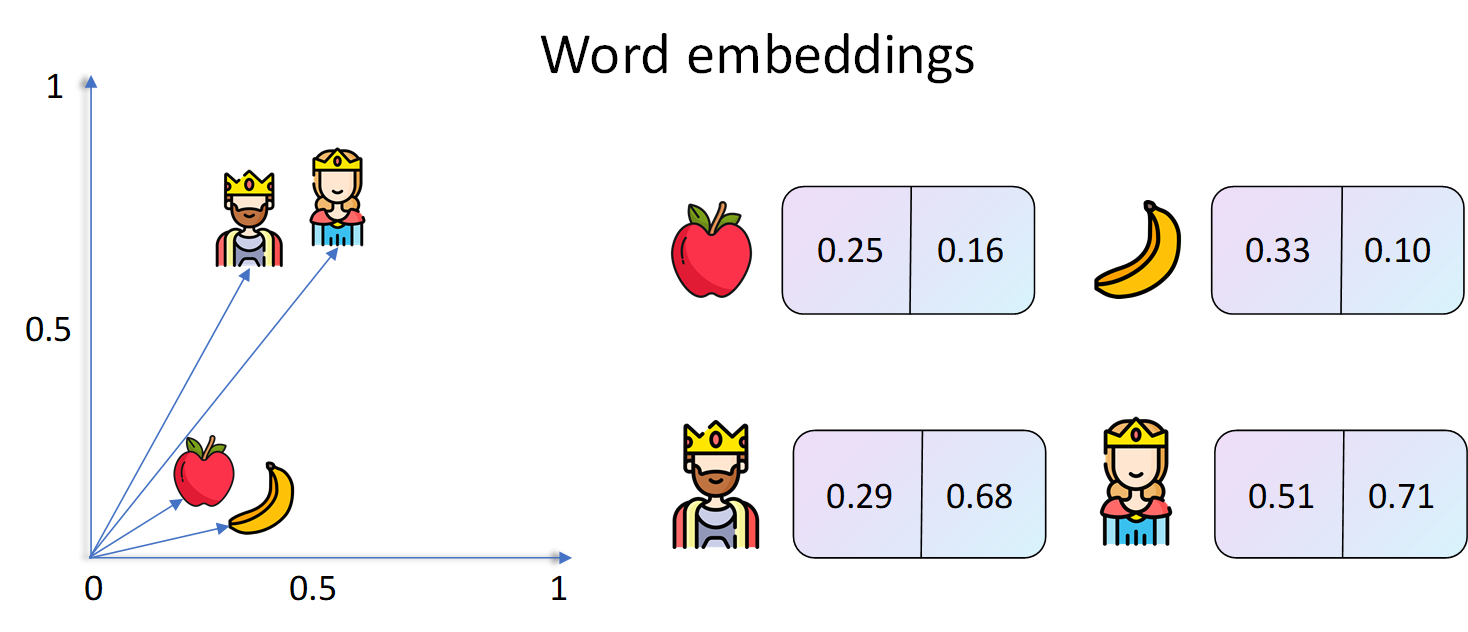
\includegraphics[width=1\textwidth]{imagenes/word_embeddings.png}
    \caption{Los vectores de palabras permiten asociar palabras mediante su cercanía dimensional, así palabras como rey o reina, o manzana y banana, se encuentran cerca en el plano.}
    \label{fig:word_embbeding}
\end{figure}

Las representaciones vectoriales de palabras han revolucionado tareas de procesamiento de lenguaje natural como la traducción automática, el análisis de sentimientos y la recuperación de información. \parencite{sentimentanalysisspanishtweets} Estas representaciones permiten a las computadoras entender el significado de las palabras y sus relaciones, lo que les permite realizar tareas lingüísticas complejas.

\subsubsection{Evaluación}

Diferentes modelos de \textit{word embeddings} generan representaciones vectoriales distintas. Sin embargo, existen algunas propiedades que todas estas representaciones deben buscar para considerarse útiles y de calidad \parencite{Wang_2019}:

\begin{itemize}
    \item No-Fusión: Los diferentes contextos locales alrededor de una palabra deben dar lugar a propiedades específicas de la palabra, como el plural o singular, los tiempos verbales, etc. Los modelos de \textit{word embeddings} deben ser capaces de discernir las diferencias en los contextos y codificar estos detalles en una representación significativa en el subespacio de la palabra. \parencite{yaghoobzadeh2016intrinsicsubspaceevaluationword}
    \item Robustez frente a la ambigüedad léxica: Deben estar representados todos los sentidos (o significados) de una palabra. Los modelos deben poder distinguir el sentido de una palabra a partir de su contexto y encontrar el embedding apropiado. \parencite{yaghoobzadeh2016intrinsicsubspaceevaluationword}
    \item Demostración de multifaceticidad: Los aspectos fonéticos, morfológicos, sintácticos y otras propiedades de una palabra deben contribuir a su representación final. Esto es importante ya que los modelos de palabras deberían generar representaciones significativas y quizás encontrar relaciones entre diferentes palabras. Por ejemplo, la representación de una palabra debería cambiar cuando se cambia el tiempo verbal o se añade un prefijo. \parencite{yaghoobzadeh2016intrinsicsubspaceevaluationword}
    \item Confiabilidad: Los resultados de un modelo de \textit{embeddings} de palabras deben ser confiables. Esto es importante ya que los vectores de palabras se inicializan aleatoriamente durante el entrenamiento. Incluso si un modelo crea representaciones diferentes del mismo conjunto de datos debido a la inicialización aleatoria, el rendimiento de varias representaciones debería ser consistente. \parencite{HellrichH17}
    \item Buena geometría: Un espacio de \textit{embeddings} debe estar correctamente distribuido. En términos generales, un conjunto pequeño de palabras frecuentes y no relacionadas debería distribuirse uniformemente en todo el espacio, mientras que un conjunto mayor de palabras raras debería agruparse alrededor de las palabras frecuentes. \parencite{GladkovaDrozd2016}
\end{itemize}

Por lo tanto, con estas propiedades en mente, se han definido varias formas de evaluar a los \textit{embeddings} resultantes de un modelo, utilizando tanto distintas tareas de NLP para evaluarlos (métodos extrínsecos) como tareas totalmente independientes a estas (métodos intrínsecos).

Uno de los métodos intrínsecos más usados es la distancia entre vectores. Al interpretar la distancia entre dos vectores como medida de similitud, se evalúa su correlación con la similitud semántica percibida por los humanos. El objetivo es medir qué tan bien las representaciones vectoriales de palabras capturan la noción de similitud percibida por los humanos y validar la hipótesis distribucional, donde el significado de las palabras está relacionado con el contexto en el que ocurren. \parencite{Wang_2019}

Un evaluador comúnmente utilizado para obtener esta métrica es la similitud coseno, definida por:

\[
\text{Similitud} = \frac{\mathbf{A} \cdot \mathbf{B}}{\|\mathbf{A}\| \|\mathbf{B}\|}
\]

Donde \( \mathbf{A} \) y \( \mathbf{B} \) son dos vectores de palabras y \( \|\mathbf{A}\| \) y \( \|\mathbf{B}\| \) son las normas 2 de los mismos. Esta prueba calcula la correlación entre todas las dimensiones de los vectores, independientemente de su relevancia para un par de palabras dado o para un grupo semántico.

Debido a que sus puntuaciones están normalizadas por la longitud del vector, es robusta frente a la escala. Además, es computacionalmente barata. Por lo tanto, es fácil comparar múltiples similitudes de un modelo y se puede usar en el prototipado y desarrollo de modelos de palabras.

Ahora, para poder medir la correlación entre dos nociones de similitud, en este caso en particular entre la noción de similitud entre los \textit{embeddings} de pares de palabras y la similitud semántica percibida por los humanos se utiliza lo que se conoce como correlación de Spearman. Esta misma examina la relación entre dos variables de una manera un poco distinta a otras correlaciones, ya que no se vale de los datos per se, sino del ranking de los mismos para ser calculada. Esto permite poder comparar dos distribuciones de datos sin importar la escala en la que se encuentren, haciendo más hincapié en su distribución dentro del ranking. En particular dadas dos distribuciones de datos, la correlación se calcula de la siguiente forma:

\[
\rho = 1 - \frac{6 \sum d_i^2}{n(n^2 - 1)}
\]

donde:
\begin{itemize}
    \item \( d_i \) es la diferencia entre los rangos de las variables \( X \) y \( Y \) para el \( i \)-ésimo par de observaciones.
    \item \( n \) es el número total de observaciones.
\end{itemize}

Esta correlación ha sido utilizada en investigaciones para poder comparar modelos de \textit{embeddings} con resultados de tareas de juicios de valor humanos, pudiendo así constatar que los \textit{embeddings} son capaces de captar similitudes entre pares de palabras de manera similar a los humanos. \parencite{chandrasekaran2021comparativeanalysiswordembeddings}

\subsubsection{Word2Vec}

Para obtener estas representaciones vectoriales, se han desarrollado un gran número de técnicas y modelos, las cuales hablaremos de algunas a continuación.

Una de las técnicas más reconocidas para la obtención de \textit{word embeddings} es la de Word2Vec. \parencite{mikolov2013efficientestimationwordrepresentations} Esta permite obtener vectores de palabras de gran calidad capaces de ser entrenados con textos de millones de palabras. Además, los vectores que representan palabras con significados similares se encuentran posicionados cerca unos de otros en este espacio de alta dimensión.

Técnicamente hablando, esta arquitectura está compuesta por una red neuronal unicapa que procesa texto al recibir lotes (\textit{batches}; es decir, subconjuntos de los datos) del mismo sin procesar, generando un espacio vectorial de varias centenas de dimensiones. Cada palabra única en los datos recibe un vector correspondiente en el espacio. La posición de estos vectores en el espacio está determinada por los significados semánticos de las palabras y su proximidad a otras palabras, en el contexto en el que los \textit{embeddings} fueron entrenados.

Esta técnica para obtener \textit{word embeddings} se puede implementar utilizando dos diseños arquitecturales: el modelo de \textit{Continuous Bag of Words} (CBOW) y el modelo \textit{Skip-Gram}. Ambos tienen como objetivo reducir la dimensionalidad de los datos y crear vectores de palabras densos, pero abordan el problema de manera diferente.

\begin{figure}[H]
    \centering
    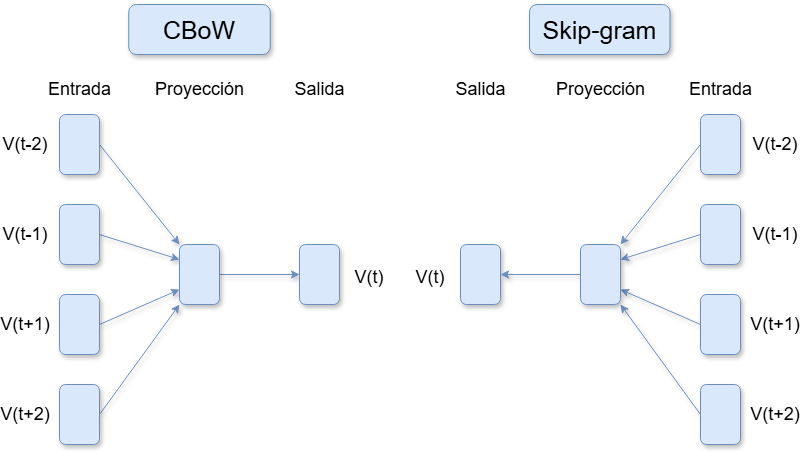
\includegraphics[width=1\textwidth]{imagenes/word2vec.drawio.png}
    \caption{Arquitecturas de Word2Vec. La arquitectura CBOW predice la palabra actual en función del contexto, mientras que Skip-gram predice las palabras circundantes dada la palabra actual.}
    \label{fig:word2vec}
\end{figure}

\sidetext{CBOW}

El modelo CBOW predice la palabra objetivo a partir de las palabras de contexto circundantes. Dicho de otro modo, utiliza las palabras del entorno para predecir la palabra en particular. Este modelo toma todas las palabras de contexto, las procesa y usa el vector resultante para predecir la palabra objetivo. Este modelo resulta beneficioso para tareas de índole más sintáctica, acompañado por un costo de computo menor. \parencite{mikolov2013efficientestimationwordrepresentations}

\sidetext{Skip-gram}

El modelo Skip-Gram predice las palabras de contexto circundante a partir de una palabra objetivo. En resumen, utiliza una sola palabra para predecir su contexto circundante.
Este modelo funciona bien para tareas más semánticas. \parencite{mikolov2013efficientestimationwordrepresentations} Sin embargo, es computacionalmente más costoso que el modelo CBOW debido a su tarea de predecir múltiples palabras de contexto.

\sidetext{Entrenamiento}

Cada palabra en el corpus se representa inicialmente como un vector de alta dimensión, previamente fijado con valores aleatorios. Estos vectores sirven como punto de partida para el proceso de entrenamiento. A medida que avanza el entrenamiento, estos vectores se actualizan en función de la función objetivo del modelo. En consecuencia, estos se posicionan más cerca entre sí en el espacio vectorial a los vectores de palabras que aparecen en contextos similares.

Otro aspecto crítico en el entrenamiento de Word2Vec es la elección del tamaño de la ventana. La ventana actúa como una ventana deslizante que pasa sobre el texto y determina qué palabras se analizan en el contexto de una palabra objetivo. Las palabras dentro de la ventana se consideran parte del contexto, mientras que las que están fuera se ignoran. La elección del tamaño de la ventana genera efectos distintos en los vectores. Un tamaño de ventana más pequeño permite que el modelo realice un aprendizaje más enfocado en la palabra objetivo, mientras que un tamaño de ventana más grande ayuda al modelo a comprender el contexto en el que fue utilizada la palabra objetivo mucho más en detalle. \parencite{levy2014} Sin embargo, un tamaño de ventana más grande aumenta la complejidad computacional del modelo, ya que se deben procesar más palabras de contexto para cada palabra objetivo.

Además, otra de las características que define a Word2Vec es la utilización de \textit{Negative Sampling}, \parencite{mikolov2013distributedrepresentationswordsphrases} el cual aborda el problema de la eficiencia computacional actualizando solo un pequeño porcentaje de los pesos del modelo en cada paso en lugar de todos ellos. Esto se logra seleccionando un pequeño número de palabras “negativas” (palabras que no están en el contexto) para actualizarlas en cada palabra objetivo.

Por último, en el modelo se realiza un submuestreo de palabras frecuentes, el cual ayuda a mejorar la calidad de los vectores de palabras. \parencite{mikolov2013distributedrepresentationswordsphrases} La idea básica es reducir el impacto de las palabras de alta frecuencia en el proceso de entrenamiento, ya que a menudo contienen información menos significativa en comparación con las palabras no frecuentes.

Al descartar aleatoriamente algunas instancias de palabras frecuentes, el modelo se ve obligado a centrarse más en las palabras raras, lo que lleva a vectores de palabras más equilibrados y con información más relevante.

\subsection{Modelos de Lenguaje}

A los \textit{embeddings} no solo los podemos encontrar como resultado de arquitecturas como Word2Vec, sino también como partes clave de otros modelos cuyo objetivo es distinto al de generar una serie de vectores de palabras; tal es el caso de algunos modelos de lenguaje, como el de la arquitectura AWD-LSTM.

Yendo más en detalle, un modelo de lenguaje es un tipo de modelo de aprendizaje automático entrenado para establecer una distribución de probabilidad sobre las palabras. Básicamente, un modelo intenta predecir la siguiente palabra más adecuada para llenar un espacio en blanco en una oración o frase, basándose en el contexto del texto dado.

\begin{figure}[H]
    \centering
    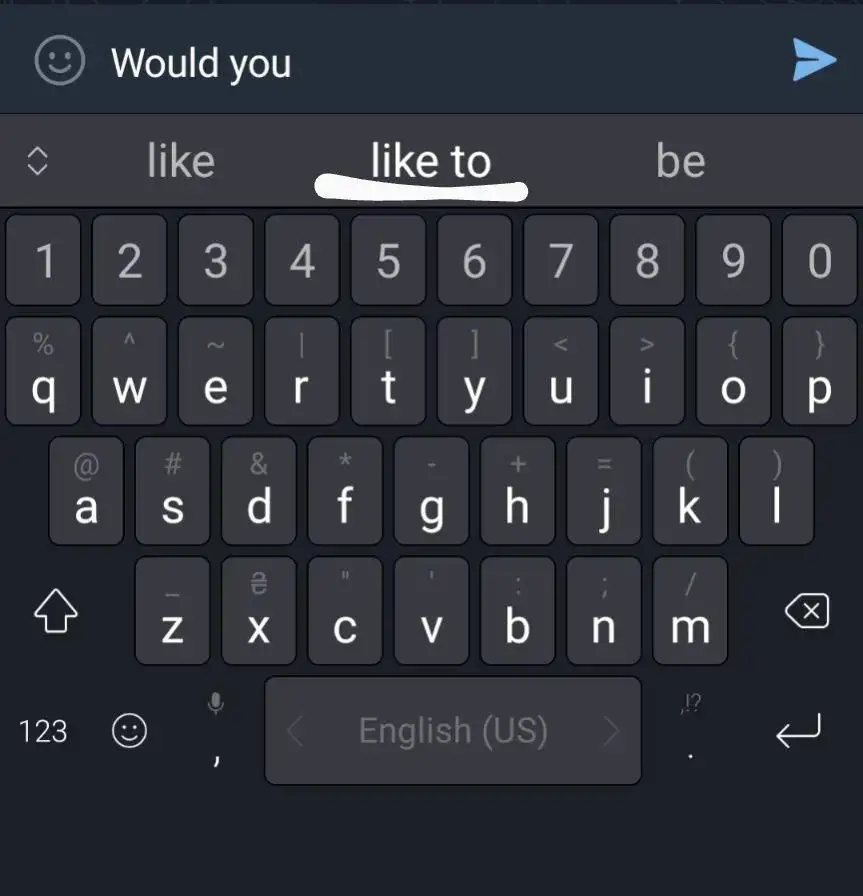
\includegraphics[width=0.5\textwidth]{imagenes/autocompletado_celular.jpg}
    \caption{Los modelos de lenguaje se utilizan en una variedad de tareas de NLP, como el reconocimiento de voz, el autocompletado de textos y la creación de resúmenes de textos.}
    \label{fig:nlp}
\end{figure}

Son un componente fundamental en el ámbito del NLP porque permiten que las máquinas comprendan, generen y analicen el lenguaje humano. Se entrenan principalmente utilizando grandes corpus de texto. Los modelos luego utilizan los patrones que aprenden de estos datos de entrenamiento para predecir la siguiente palabra en una oración o generar nuevo texto que sea gramaticalmente correcto y semánticamente coherente.

Existen diferentes tipos de Modelos de Lenguaje, los cuales se pueden clasificar en dos categorías: \textbf{modelos estadísticos} y modelos basados en \textbf{redes neuronales profundas}.

Por un lado, los modelos estadísticos de lenguaje son un tipo de modelo que utilizan patrones estadísticos en los datos para hacer predicciones sobre la probabilidad de secuencias específicas de palabras. Por ejemplo, un enfoque básico para construir un modelo de lenguaje probabilístico es la utilización de n-gramas.

Por otro lado, los modelos de lenguaje neuronales, como su nombre indica, utilizan redes neuronales para predecir la probabilidad de una secuencia de palabras. Estos modelos se entrenan con un gran corpus de datos de texto y cumplen el objetivo de predecir palabras dado un contexto al minimizar una función de costo.

\begin{figure}[H]
    \centering
    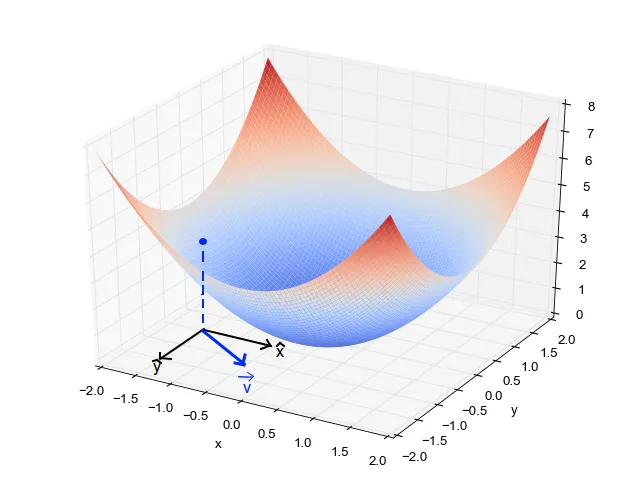
\includegraphics[width=0.8\textwidth]{imagenes/function.jpg}
    \caption{La idea general de los modelos basados en redes neuronales es minimizar una función de costo generada a partir de los pesos de la red. Para esto se calcula el gradiente de la función en un punto, o sea la pendiente de la tangente a la función de coste. Este gradiente puede ser calculado de a batches o de a una entrada a la vez, o sea de manera estocástica.}
    \label{fig:gradiente}
\end{figure}

Una vez entrenados estos modelos, los mismos permiten captar mejor dependencias de largo alcance entre palabras que con los modelos estadísticos tradicionales. \parencite{Wang2017ngram} Por ejemplo, al utilizar un modelo estadístico basado en n-gramas, el contexto que presenta el modelo es limitado, mientras que los modelos basados en redes neuronales presentan diversidad de estrategias para poder recordar contextos lejanos a lo largo del entrenamiento. Esta es la razón por la cual nos decantamos por ellas. Una de las arquitecturas más reconocidas que utiliza estas estrategias son las Redes neuronales recurrentes (RNNs).

\subsubsection{Redes neuronales recurrentes}

Una red neuronal recurrente, o RNN, es una red neuronal profunda entrenada con datos secuenciales o de series temporales para crear un modelo de aprendizaje automático que pueda hacer predicciones o conclusiones basadas en estas mismas.

\begin{figure}[H]
    \centering
    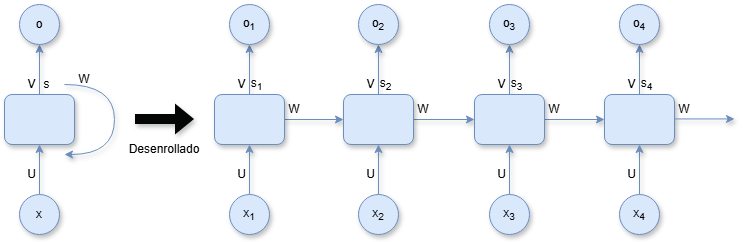
\includegraphics[width=1\textwidth]{imagenes/RNN.drawio.png}
    \caption{Diagrama de una Red neuronal recurrente mostrando su versión compacta a la izquierda y su versión desenrollada a la derecha, ilustrando cómo la red se expande a lo largo del tiempo para procesar secuencias de datos.}
    \label{fig:rnn}
\end{figure}

Se distinguen por su “memoria”, ya que toman información de entradas anteriores para influir en la entrada y salida actuales. Mientras que las redes neuronales profundas tradicionales suponen que las entradas y salidas son independientes entre sí, la salida de las redes neuronales recurrentes depende de los elementos anteriores dentro de la secuencia. Incluso existen tipos de RNNs cuya salida actual no solo se ve influenciada por los resultados anteriores sino también por los resultados futuros.

Otra característica distintiva de las redes recurrentes es que comparten parámetros en cada capa de la red. Mientras que las redes tradicionales tienen diferentes pesos en cada nodo, las redes neuronales recurrentes comparten pesos en cada capa de la misma. Dichos pesos se ajustan a través de los procesos de \textit{backpropagation} y descenso por el gradiente para facilitar el aprendizaje.

Las redes neuronales recurrentes utilizan algoritmos de \textit{backpropagation} a través del tiempo (BPTT, de sus siglas en inglés) para determinar los gradientes, lo cual es ligeramente diferente del algoritmo tradicional, ya que es específico para datos secuenciales. Los principios de BPTT son los mismos que los de \textit{backpropagation} tradicional, donde el modelo se entrena calculando errores desde su capa de salida hacia la capa de entrada. Estos cálculos permiten ajustar y adaptar los parámetros del modelo adecuadamente. La diferencia con el enfoque tradicional es que BPTT suma los errores en cada paso temporal, mientras que las redes normales no necesitan hacerlo, ya que no comparten parámetros entre las capas.

Este tipo de redes, sin embargo, se ven afectadas por diversas cuestiones. Una de ellas, aunque no de manera tan tajante como puede ser en el caso de los modelos basados en n-gramas, es la incapacidad de recordar dependencias a largo plazo; es decir, si el estado anterior que influye en la predicción actual no está en el pasado reciente, el modelo RNN puede no ser capaz de predecir correctamente el estado actual.

Por ejemplo, supongamos que queremos predecir las palabras en la siguiente oración:

\begin{center}
    ...\hlred{Alicia es alérgica a} \hlorange{los frutos secos. Ella} \hlyellow{no puede comer nueces}...
\end{center}

El contexto de una alergia a los frutos secos nos ayuda a anticipar que el alimento que no se puede comer contiene frutos secos. Sin embargo, si ese contexto se mencionara varias oraciones antes, sería difícil para la RNN inferir esa información, debido a su falta de capacidad para asociar relaciones entre oraciones muy distantes.

A su vez, se considera que las RNNs, las cuales en su mayoría dividen la información del dataset en batches de tamaño fijo,  presentan algunos inconvenientes a la hora de manejar la información de entrenamiento de manera eficiente. Esto se debe a que al utilizar un tamaño fijo para el batch, independientemente en la época que esté del entrenamiento, siempre van a existir un grupo de elementos del batch los cuales no van a poder aprovecharse de la capacidad recurrente de la red. Por ejemplo, volviendo al caso de la oración anterior, si entrenáramos nuestro modelo con batches de tamaño 4, nos pasaría que palabras como ‘Alicia’, ‘los’ y ‘no’ no se aprovecharían de la información previa a ellas, a pesar de ser esto una pieza clave de las RNN. \parencite{merity2017regularizingoptimizinglstmlanguage}

Al mismo tiempo, durante este proceso, las RNN tienden a enfrentar otros dos problemas, conocidos como \textit{exploding gradients} y \textit{vanishing gradients}. Estos problemas se definen por el tamaño del gradiente. Cuando el gradiente es demasiado pequeño, este mismo sigue disminuyendo hasta que los parámetros de peso se vuelven insignificantes, y en ese punto, el algoritmo deja de aprender. Por otro lado, los gradientes que explotan ocurren cuando el gradiente es demasiado grande, creando un modelo inestable. En este caso, los pesos del modelo crecerán demasiado y eventualmente se llegará a problemas de convergencia.

Una solución utilizada para mitigar estos problemas, especialmente el de los gradientes altos, es la implementación del concepto de \textit{gradient clipping}, el cual se basa en la idea de establecer un límite, el cual si es pasado por el gradiente durante el entrenamiento se procede a reducir proporcionalmente el mismo para evitar que el vector se vuelva demasiado grande. \parencite{pascanu2013difficultytrainingrecurrentneural} A su vez también han surgido otras arquitecturas de modelos de lenguaje que buscan afrontar estos problemas.

\subsubsection{LSTM}

Las LSTMs (proveniente del inglés, \textit{Long Short-Term Memory}) son una serie de arquitecturas populares de RNNs surgidas con el objetivo de solucionar el problema del \textit{exploding gradients} y \textit{vanishing gradients}. Además, con esta arquitectura se busca resolver otros inconvenientes como el de la incapacidad de asociar dependencias a largo plazo. \parencite{lstm}

Para solucionar esto, las redes LSTM introducen un nuevo tipo de células de memoria, distintas a las presentes en las RNNs y capaces de retener información a lo largo de secuencias extensas. Cada célula de memoria presenta tres componentes principales: una puerta de entrada, una puerta de olvido y una puerta de salida. Estas puertas ayudan a regular el flujo de información dentro y fuera de la célula de memoria.

\begin{figure}[H]
    \centering
    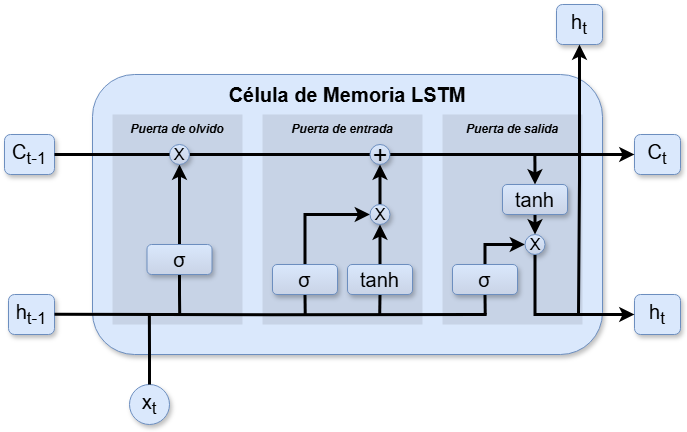
\includegraphics[width=1\textwidth]{imagenes/LSTM.png}
    \caption{Diagrama de una LSTM junto a sus puertas. Las LSTM utilizan estas para regular el flujo de información, lo que les permite aprender dependencias a largo plazo en los datos, haciéndolas particularmente efectivas para tareas que involucran datos secuenciales como la predicción de series temporales, el procesamiento del lenguaje natural, el reconocimiento de voz, y más.}
    \label{fig:lstm}
\end{figure}

\begin{itemize}
    \item \textbf{La puerta de entrada} determina cuánta de la nueva información debe almacenarse en la célula de memoria. Toma la entrada actual y el estado oculto anterior como entradas, y genera un valor entre 0 y 1 para cada elemento de la célula de memoria.
    \item \textbf{La puerta de olvido} decide qué información debe descartarse de la célula de memoria. Al igual que la puerta de entrada, toma la entrada actual y el estado oculto anterior y emite un valor entre 0 y 1. Un valor de 0 significa que la información se ignora, mientras que un valor de 1 indica que se retiene.
    \item \textbf{La puerta de salida} controla cuánta de la información de la célula de memoria debe usarse para calcular el estado oculto. También toma la entrada actual y el estado oculto anterior como entradas y emite un valor entre 0 y 1 para cada elemento de la célula de memoria.
\end{itemize}

Al controlar y memorizar información a lo largo de secuencias largas, las LSTM pueden mitigar los problemas de \textit{exploding gradients} y \textit{vanishing gradients}, permitiendo un entrenamiento más efectivo y una mejor captura de patrones a largo plazo en los datos secuenciales.

Durante los años, muchas arquitecturas han florecido utilizando a las LSTM como base, ya sea como motivación o literalmente. Por ejemplo, una de ellas son las GRU, o \textit{Gated Recurrent Units} de sus siglas en inglés, las cuales tenían como objetivo presentar una alternativa que pudiera solucionar los problemas resueltos por las LSTM, con la ventaja de tener un diseño más simple y una complejidad computacional mucho menor. Esto lo lograban, entre otras cosas, condensando el trabajo de las compuertas de entrada y olvido de la LSTM en una sola compuerta llamada compuerta de actualización. \parencite{chung2014empiricalevaluationgatedrecurrent} Sin embargo, si dejamos de lado la rapidez para entrenar los modelos, las GRU generan peores resultados que las LSTMs fuera de datasets pequeños. \parencite{lstmandgru}

\subsubsection{AWD-LSTM}

\label{sec:awd-lstm}

Otro ejemplo de modelo de lenguaje basado en LSTMs es la AWD-LSTM (de sus siglas en inglés, \textit{ASGD Weight-Dropped LSTM}). A diferencia de la arquitectura LSTM básica, la AWD-LSTM implementa varias técnicas de regularización a lo largo de su red neuronal, con el objetivo de mejorar la capacidad predictiva del modelo, especialmente en la capacidad del modelo para poder generalizar. Además, estas técnicas mejoran la estabilidad del modelo, ya que reducen la probabilidad de sobreajuste del mismo.

\begin{figure}[H]
    \centering
    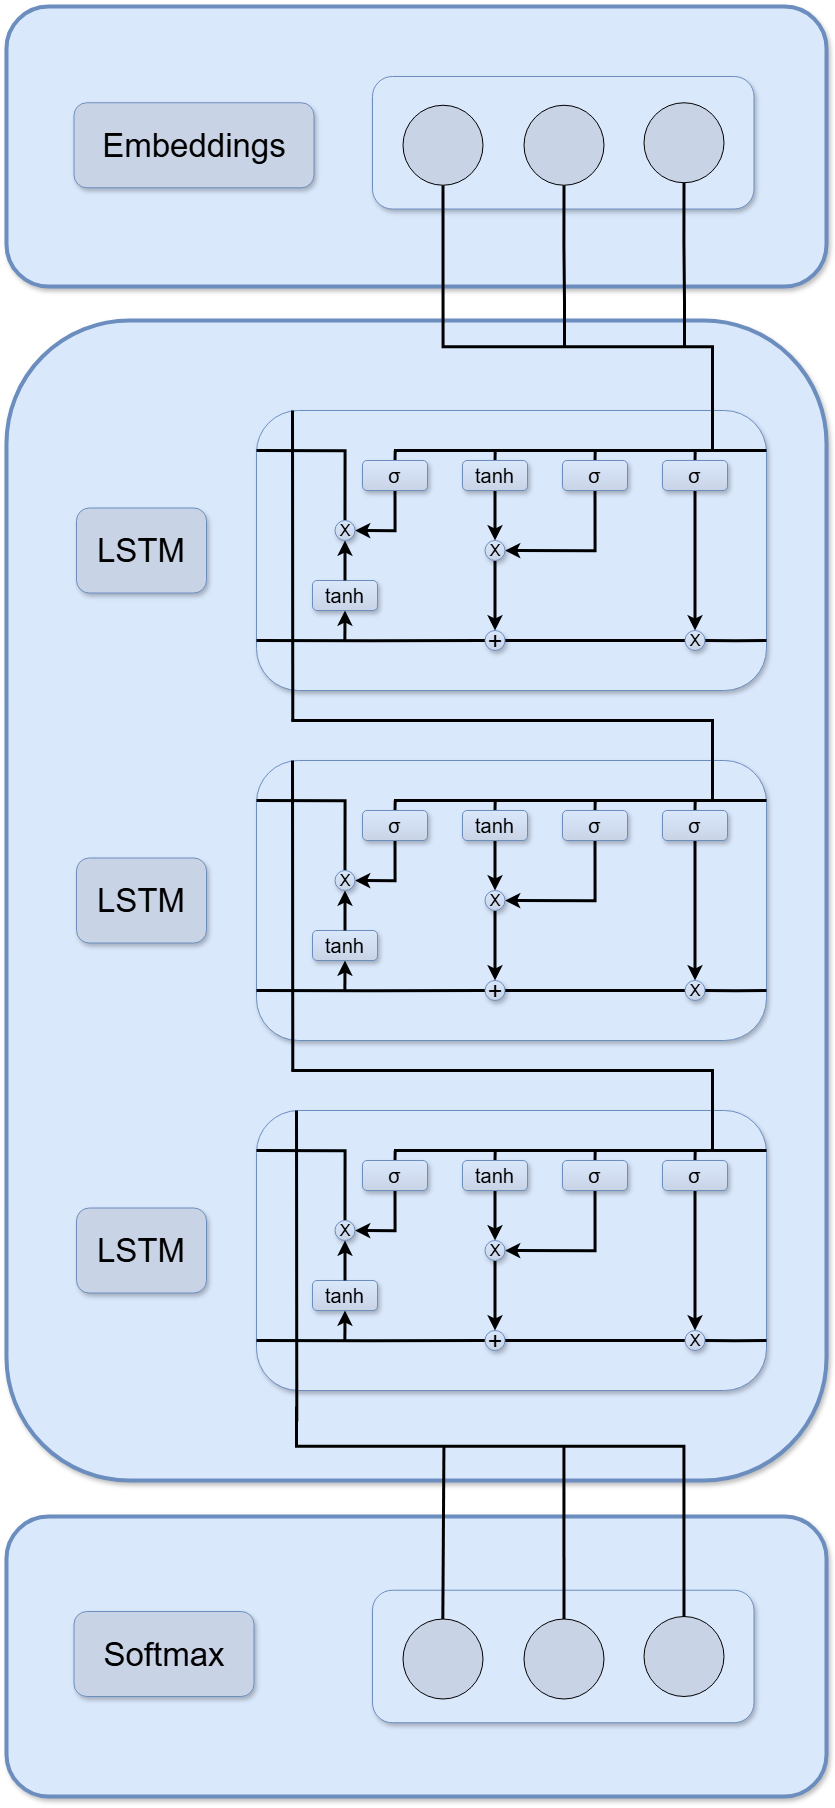
\includegraphics[width=0.42\textwidth]{imagenes/AWD-LSTM.drawio.png}
    \caption{Estructura clásica de un modelo basado en AWD-LSTM. El mismo presenta una capa de \textit{embeddings}, por el cual la entrada pasará y verá sus palabras transformadas en vectores de palabras. Unas 3 células LSTM y una capa softmax la cual permite obtener la distribución de probabilidades para la siguiente palabra del texto dado el vocabulario.}
    \label{fig:awd-lstm}
\end{figure}

Muchas de estas técnicas de regularización están asociadas a la aplicación de \textit{dropout} en porcentajes distintos en distintas partes de la red neuronal. Estas partes en concreto son:

\begin{itemize}
    \item En la capa de \textit{embeddings}, los pesos de algunas palabras dentro del vocabulario de la capa son desactivados.
    \item Luego de la capa de \textit{embeddings}, una vez obtenidos los \textit{embeddings} de todas las palabras del texto de entrada, ciertos pesos de los vectores son desactivados de manera aleatoria.
    \item Previo al ingresar a cada celda LSTM.
    \item Dentro de cada una de las celdas LSTM.
    \item Al finalizar la activación de la última celda.
\end{itemize}

Adicionalmente, la arquitectura introduce un algoritmo de optimización nuevo, llamado NT-ASGD (de sus siglas \textit{Non-monotonically Triggered Averaged Stochastic Gradient Descent}). En resumen, se implementa un algoritmo parecido al de descenso por el gradiente estocástico, con la diferencia de que los pesos de la red no se ven afectados solamente por el gradiente actual, sino por el promedio de los últimos n gradientes, donde n es un hiperparámetro. Además, este promedio no se realiza a partir del primer batch de entrada, sino que el algoritmo actúa como un descenso por el gradiente estocástico normal hasta que el modelo empeora o se estanca durante varias entradas seguidas, a partir del cual se empieza a calcular el gradiente final en base al promedio de los anteriores hasta finalizar el entrenamiento.

Asimismo, anteriormente habíamos mencionado que las RNNs podían llegar a no ser 100\% eficientes en el uso del dataset de entrenamiento, debido a que, en el caso de las tareas de predicción de texto, existen algunas palabras que no aprovechan la capacidad recurrente de la red si se utiliza un tamaño de batch fijo durante el entrenamiento. Este problema es atacado por la AWD-LSTM variando el tamaño del batch que se utiliza en cada época. En particular esta variación la realiza partiendo de un tamaño base, el cual llamaremos $seq$. En un primer paso, se elige como valor intermedio con probabilidad $p$ a este valor $seq$ y con probabilidad $1-p$ a $\frac{seq}{2}$, con $p$ un valor muy cercano a 1. Esto se hace para aumentar el rango de valores usados durante el entrenamiento. Para finalizar, se selecciona el tamaño de batch final a partir de una distribución normal con media en ese valor intermedio y un desvío estándar. De esta manera, se aprovecha mucho más la capacidad recurrente de la AWD-LSTM.

Por último, el \textit{learning rate} del modelo es re-escalado dependiendo del tamaño de batch resultante, ya que se ha encontrado una tendencia a favorecer a las oraciones más cortas durante el entrenamiento si se utiliza un tamaño de batch variable junto a un \textit{learning rate} fijo. \parencite{merity2017regularizingoptimizinglstmlanguage}

Debido a estas mejoras introducidas por esta arquitectura y porque fue una de las más populares previo al surgimiento de otros modelos como los \textit{transformers}, decidimos tomar a la AWD-LSTM como nuestro eje principal en ese trabajo.

\subsubsection{Evaluación}

Una vez se tiene elegido el tipo de arquitectura de modelos de lenguaje que se utilizara para llevar a cabo nuestro propósito, es lógico preguntarse de qué manera podemos evaluar nuestros modelos para ver si se comportan de manera satisfactoria y son capaces de comprender el lenguaje humano.

Para esto, fuera de las típicas métricas utilizadas para evaluar modelos de aprendizaje automático como el \textit{Accuracy} o el \textit{F1 Score}, existen otras, como la \textit{Perplexity}, la cual es considerada como una medida utilizada para cuantificar la incertidumbre asociado con una distribución de probabilidad. Esta métrica a lo largo de los años se ha utilizado como una manera de evaluar distintos modelos de lenguaje. \parencite{merity2017regularizingoptimizinglstmlanguage}

Yendo más en detalle, esta métrica se define como la exponenciación de la entropía de una distribución de probabilidad. Se puede expresar como:

\[
PP(W) = 2^{H(W)}
\]

donde el $H(W)$ es la entropía del modelo con respecto a la secuencia de palabras $W$. Un nivel de \textit{perplexity} más bajo indica un mejor modelo predictivo, ya que implica que el modelo tiene más confianza en sus predicciones. Por el contrario, un nivel de \textit{perplexity} más alto sugiere una mayor incertidumbre y predicciones menos efectivas.

\section{Movimientos oculares durante la lectura}

La lectura se puede considerar como un desarrollo relativamente reciente en la historia de la humanidad, existiendo sólo desde hace unos pocos miles de años. \parencite{ImmordinoYangDeacon2007} Sin embargo, se ha convertido en una habilidad esencial en la vida moderna, que se desarrolla a lo largo de años de exposición, instrucción formal y práctica.
Una buena habilidad de lectura es fundamental para el logro académico (para una discusión, ver \textcite{Renadya}), y para los estudiantes de un segundo idioma, la lectura es una puerta de entrada para aprender nuevo vocabulario, más lenguaje coloquial y nuevas construcciones gramaticales. \parencite{wilkinson}

Sabemos que para los lectores el objetivo principal es identificar palabras, comprender su significado e integrarlas en su comprensión progresiva de una oración y/o de un discurso más amplio. Sin embargo, ¿Qué ocurre exactamente cuando leemos? ¿Cómo se mueven nuestros ojos?

Tal y como menciona \textcite{Brown1895}, nuestros ojos a la hora de leer se asemejan al movimiento del segundero dentro de un reloj, se realiza un tirón y una pequeña pausa, luego otro tirón, y así sucesivamente; solo que nuestros ojos no son tan regulares, los tirones a veces tienen una amplitud mayor o menor, y las pausas varían en duración, aunque, a menos que hagamos un esfuerzo, siempre son breves. Durante los tirones prácticamente no vemos nada, por lo que no tenemos ante nosotros un panorama en movimiento, sino una serie de imágenes fijas que se suceden rápidamente.

Estos “tirones” del ojo — en otras palabras, sus movimientos — son lo que comúnmente denominamos sacadas. El intervalo entre los movimientos de los ojos, cuando estos se detienen, se llama fijación. Ambos son un tipo de respuesta fisiológica automática, lo que significa que no están bajo nuestro control consciente. \parencite{Rayner2012} Cualquier secuencia completa de estos dos se denomina como un \textit{scanpath}. Sin embargo, al leer, las sacadas no siempre mueven el ojo hacia adelante en el texto. Aproximadamente entre el 10 y el 15 por ciento de las veces, los lectores mueven los ojos hacia atrás (regresan) a secciones del texto previamente vistas. Estos movimientos hacia atrás se conocen como regresiones. Las regresiones pueden ser cortas o largas. Las regresiones cortas suelen deberse a un exceso de movimiento sobre el objetivo. Por otro lado, las regresiones largas son atribuidas comúnmente a la dificultad del texto leído, que puede deberse a diversos factores.

Básicamente, cuando leemos o miramos una escena o imagen, nuestros ojos se detienen para procesar la información en esa ubicación y luego se mueven a otro punto donde hay otra información disponible. Durante las fijaciones, el sistema cognitivo percibe y procesa la información visual, además de planificar cuándo y hasta dónde mover los ojos a continuación. En la mayoría de las circunstancias normales, durante un movimiento sacádico, los ojos se mueven tan rápido que no obtenemos nueva información visual. \parencite{Rayner2009} Sin embargo, mientras no se codifica nueva información visual durante los movimientos sacádicos, el procesamiento de la información ya percibida previamente continua. \parencite{Irwin1998} \parencite{Irwin1996}

Entonces, ¿de qué manera podría interesar el rastreo y medición de los movimientos oculares de las personas dentro de la lectura? Las fijaciones, los movimientos sacádicos y las regresiones ocurren generalmente de forma “automática”, sin que seamos conscientes de ello. De esta forma, el seguimiento de los movimientos oculares nos ofrece una ventana a un comportamiento en gran medida inconsciente. Además, se ha demostrado que en tareas de procesamiento complejo, como es el caso de la lectura, la ubicación de los ojos proporciona un índice de atención. \parencite{Rayner2009} Esto significa que nuestros ojos indican en qué estamos prestando atención y cuánta energía cognitiva se está invirtiendo para procesar la información en el punto de fijación. Así, la dificultad y la complejidad de lo que miran los ojos influyen en las fijaciones y los movimientos sacádicos. \parencite{CastelhanoRayner2008} Cuando el estímulo es más difícil, aumentan las duraciones de fijación y las regresiones, mientras que el tamaño de los movimientos sacádicos disminuye. Esto significa que, en la lectura, los textos más difíciles provocan fijaciones y regresiones más frecuentes y prolongadas, mientras que los sacádicos se acortan. Al observar escenas o imágenes más densas o complejas, las fijaciones también se alargan y los movimientos sacádicos se acortan.

Estas, en definitiva, son algunas de las razones por las cuales el análisis de movimientos oculares se ha vuelto una de las herramientas más poderosas para estudiar la manera en que la información visual es procesada por la mente humana y una de las herramientas más estándares a la hora de realizar estudios sobre lectura en los campos de la psicolingüística, la psicología cognitiva y la lingüística aplicada. \parencite[p. 1474]{Rayner2009} Sin embargo, cabe aclarar que todas estas ventajas brindadas por el análisis de los movimientos oculares se apoyan en gran medida en lo que se conoce como la hipótesis ojo-mente, la cual afirma que hay una estrecha relación entre los movimientos del ojo y el procesamiento cognitivo dentro de nuestro cerebro a la hora de leer. \parencite{JustCarpenter1980} A su vez, esta hipótesis se basa en dos ideas subyacentes:

\begin{enumerate}
    \item Primero, está la suposición de que lo que se está fijando es lo que se está considerando. Esto significa que cuando los ojos se fijan en una palabra “x”, el cerebro está trabajando para descifrar y entender esta palabra y no otra palabra “z” que apareció tres palabras antes. Es decir, los lectores intentan interpretar las palabras a medida que las encuentran. No obstante, esta suposición termina resultando ser, aunque acertada, algo simplista. \parencite{EhrlichRayner1983} Por ejemplo, en una oración como “Maria vendió su caballo a José porque ella decidió dejar de montar”, cuando los ojos se posan en la palabra “ella”, para interpretarla, el cerebro necesita considerar entidades previamente encontradas que podrían ser referentes potenciales del pronombre. Así, cuando los ojos se detienen en “ella”, la mente está trabajando en esta palabra; sin embargo, también considera elementos previos de la oración que podrían ser referentes potenciales (por ejemplo, “Maria”).
    \item La segunda parte, por otra parte, estipula que la cantidad de tiempo dedicado a fijar un elemento o región refleja el esfuerzo cognitivo necesario para procesarlo. Esto significa que fijaciones más largas y frecuentes indican un mayor esfuerzo de procesamiento, y las fijaciones más breves y/o los saltos indican un menor esfuerzo de procesamiento. Además, es importante aclarar que estos tiempos deben tomarse en términos relativos: una mayor o menor duración y un mayor o menor esfuerzo de procesamiento deben compararse con algo. En general, el esfuerzo cognitivo se decide asociar a una región de interés en particular (conocida como ROI, de sus siglas en inglés)
\end{enumerate}

\subsection{Métricas asociadas a movimientos oculares}

\label{subsec:metricas_movimientos}

Habiendo previamente mencionado todas las ventajas de la utilización de movimientos oculares para obtener información sobre el comportamiento inconsciente de las personas a la hora de leer, parecería lógico preguntarse de qué manera se puede extraer esta información.

A partir de esto, la tecnología de seguimiento ocular nos permite indicar, entre otras cosas, dónde se posan los ojos de las personas, cuántas veces se posan en esa posición o región (conteo de fijaciones) y cuánto dura cada fijación (duración de fijación), además de medir la duración y la longitud de los movimientos sacádicos. Estas medidas se toman en experimentos utilizando el equipamiento adecuado, dividiendo los mismos en distintas pruebas, donde el equipamiento va recolectando información sobre los movimientos oculares de un sujeto a medida que este va realizando la lectura de un corpus de texto.

Ahora, dado que las fijaciones (y específicamente la duración de las mismas) son más sensibles a los factores lingüísticos que los movimientos sacádicos \parencite{StaubRayner2007}, estas tienden a ser las métricas que más nos interesan en estudios basados en textos. Estas métricas se clasifican en “tempranas”, “intermedias” o “tardías” y se entiende que reflejan diferentes etapas del procesamiento de la lectura. Las medidas tempranas se consideran principalmente como un reflejo de procesos automáticos de reconocimiento de palabras y acceso léxico, mientras que las medidas tardías tienden a reflejar procesos más conscientes, controlados y estratégicos. (\cite{Altarriba1996}; \cite{Inhoff1984}; \cite{Paterson1999}; \cite{StaubRayner2007})

\begin{figure}[H]
    \centering
    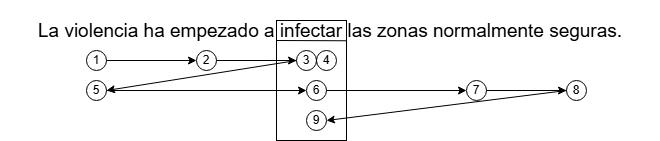
\includegraphics[width=1\textwidth]{imagenes/scanpath.png}
    \caption{Ejemplo de scanpath. Cada círculo debajo de una palabra indica una fijación en el orden el cual fue hecha mientras que las flechas indican las sacadas realizadas. En este caso la palabra crítica tenida en cuenta es “infectar”.}
    \label{fig:scanpath}
\end{figure}

\subsubsection{Métricas tempranas}

Cada una de estas métricas puede considerarse como un índice de acceso léxico, o de qué tan fácilmente se reconoce y se recupera la palabra del léxico mental. Algunos factores que se sabe que afectan estas métricas incluyen la frecuencia y familiaridad de la palabra, la ambigüedad de significado, la predictibilidad y la asociación semántica.

\begin{itemize}
    \item \textit{Skipping Rate}: Se utiliza para determinar la proporción de palabras que no reciben fijación, o sea las palabras que son salteadas durante la primera pasada de lectura. Esta métrica se suele reportar como una probabilidad (o porcentaje) y se calcula como el número total de pruebas en los que la palabra se omitió durante la primera pasada de lectura dividido el número total de pruebas. Por ejemplo, en el scanpath de arriba vemos que la palabra crítica no fue salteada, por lo que esta prueba contribuiría a la cantidad total de pruebas pero no al numerador de la división.
    \item \textit{First Fixation Duration}: Ó FFD proveniente de su acrónimo en inglés, se refiere al tiempo de la primera fijación realizada en una palabra o región de interés. En el caso de ejemplo se consideraría solamente el tiempo de la fijación número 3.
    \item \textit{Single Fixation Duration}: Métrica muy parecida a la anterior, con la diferencia de que solo se tienen en cuenta las pruebas donde se ha realizado una sola fijación sobre la palabra en cuestión o ROI. En el caso de la palabra crítica en el ejemplo no se vería contada al presentar más de una fijación.
    \item \textit{First Pass Reading Time}: También conocida como \textit{Gaze Duration} o FPRT, considera todas las fijaciones hechas en una palabra o ROI antes de que la mirada salga (ya sea a la izquierda o a la derecha) de la misma. Dentro del ejemplo presentado, la suma se realizaría entre los tiempos de las fijaciones 3 y 4.
\end{itemize}

\subsubsection{Métricas intermedias}

Existen métricas que son difíciles de clasificar como tempranas o tardías, como las relacionadas a las regresiones dentro de la lectura, ya que pueden indicar dependiendo de cómo se las utilice como dificultad al encontrar un elemento por primera vez, así como el tiempo posterior necesario para superar esa dificultad. \parencite{CliftonStaubRayner2007}

\begin{itemize}
    \item \textit{Regression Path Duration}: también conocida como \textit{go past time}, es una medida del tiempo dedicado a la palabra en sí y a cualquier parte anterior de la oración antes de que el lector avance más allá de la palabra crítica hacia la derecha. También se puede medir una métrica parecida en términos de cantidad o como un porcentaje, es decir, cuántas pruebas tuvieron una regresión dentro del ROI. Volviendo al ejemplo, la métrica en este caso estaría compuesta por la suma de la duración de las fijaciones 3, 4, 5 y 6.
\end{itemize}

\subsubsection{Métricas tardías}

Las medidas tardías pueden no reflejar factores puramente léxicos y estar más influenciadas por propiedades contextuales, sintácticas o de nivel de discurso de lo que se está leyendo. Por ejemplo, la ambigüedad sintáctica puede llevar a fijaciones más prolongadas en una palabra o región crítica, así como a más regresiones al contexto anterior a medida que el lector se ve obligado a reevaluar el análisis inicial. \parencite{FrazierRayner1982}

\begin{itemize}
    \item \textit{Total Reading Time}: Es la suma de todas las fijaciones realizadas en una palabra o ROI durante un ensayo. En el ejemplo, el \textit{Total Reading Time} de la palabra crítica sería la suma de las fijaciones 3, 4, 6 y 9.
    \item \textit{Re-reading Time}: Existen diferentes definiciones de la misma dentro de la literatura. Una de ellas se calcula a partir de la resta entre dos métricas anteriormente mencionadas, el \textit{Regression Path Duration} menos el \textit{First Pass Reading Time}. Abstrayendo al caso en particular, haciendo la resta de las dos métricas previas se tendría que el \textit{Re-reading Time} es la suma de la fijación 5 y 6.
    \item \textit{Second Pass Reading Time}: Se define como la suma de todas las fijaciones dentro de un ROI luego de haber abandonado la región de interés por primera vez. En el caso de ejemplo, la suma se realizaría entre las fijaciones 6 y 9.
    \item \textit{Fixation Count}: Cantidad de fijaciones realizadas sobre un ROI. En este caso, un total de 4 fijaciones sobre la palabra crítica.
\end{itemize}

Es fundamental recordar que las medidas no son independientes entre sí: \textit{First Fixation Duration} es parte de \textit{First Pass Reading Time}, que a su vez es parte de \textit{Total Reading Time}. De manera similar, \textit{Total Reading Time} y \textit{Fixation Count} generalmente están altamente correlacionados. Por lo tanto, a la hora de utilizar estas métricas, el objetivo debe ser analizar una gama de medidas para investigar el patrón general, y si un efecto sólo aparece en una de nuestras medidas, esto debe interpretarse con precaución.

\section{Movimientos oculares en NLP}

A medida que los modelos de NLP se vuelven cada vez más frecuentes en la sociedad, los investigadores han visto la necesidad de buscar maneras de cómo mejorar estos modelos, por ejemplo aprovechando información recopilada de manera pasiva de los lectores humanos, como las señales de movimientos oculares.

Esto genera que recientemente los movimientos oculares hayan incursionado en el campo de NLP, a partir de las relaciones existentes entre la duración de la mirada sobre las palabras (\textit{gaze duration}) y la capacidad de predecirlas (\cite{Rayner1998}, \cite{Reinhold2006}). Particularmente, se realizaron análisis sobre los modelos del lenguaje en conjunto a datos de MO para capturar la relación entre ellos (\cite{Bianchi2020}, \cite{Hofmann2017}), revelando información sobre la influencia de otras variables (como la frecuencia de la palabra) y permitiendo obtener una mejor comprensión de qué mecanismos actúan en el cerebro en determinado momento. Otros trabajos se han enfocado en la incorporación de los datos de MO para mejorar los modelos del estado del arte, en campos como el etiquetado de palabras (\textit{Part of Speech Tagging}) \parencite{barrett-etal-2016-weakly}, compresión de oraciones (\textit{Sentence compression}) \parencite{klerke2016improvingsentencecompressionlearning}, traducción automática (\textit{Machine translation}) \parencite{sajjad-etal-2016-eyes}, análisis de sentimiento (\textit{Sentiment analysis}) \parencite{mishra2017} y reconocimiento de entidades nombradas (\textit{Named-entity Recognition}). \parencite{hollenstein2019} En todos los casos, se observaron mejoras frente a los modelos que no tenían en consideración estos datos.

Curiosamente, la manera de incorporar esta información cognitiva a los modelos de NLP varía según el caso, por ejemplo existen casos en donde la información es concatenada a los \textit{embeddings} del modelo \parencite{hollenstein2019}, mientras que en otros casos se aprovecha de un tipo de entrenamiento conocido como aprendizaje multitarea. \parencite{klerke2016improvingsentencecompressionlearning}

\subsection{Aprendizaje Multitarea}

¿En qué consiste entonces esta técnica? El aprendizaje multitarea (MTL, por sus siglas en inglés) consiste en entrenar una red neuronal para ejecutar múltiples tareas compartiendo algunas de las capas y parámetros de la red entre las mismas. El objetivo es mejorar la capacidad de generalización del modelo aprovechando la información compartida entre las tareas, prediciendo varias cosas a la vez. \parencite{Caruana1997}

\begin{figure}[H]
    \centering
    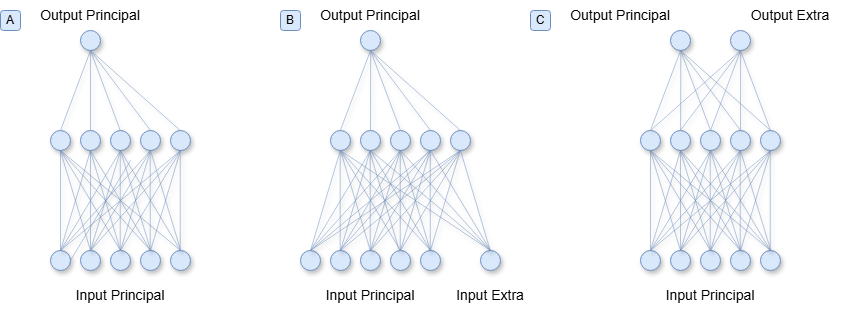
\includegraphics[width=1\textwidth]{imagenes/multitarea.png}
    \caption{Aprendizaje multitarea como es descrito por \textcite{Caruana1997}. La red neuronal A es una red estándar la cual no utiliza ningún tipo de información extra. Por otro lado la red B incorpora comportamiento extra añadiendolo como input de la red. En el caso de la red C se aplica el aprendizaje multitarea: el comportamiento extra es añadido como output de la red y no como input.}
    \label{fig:multitarea}
\end{figure}

Llevándolo al ámbito de NLP con la utilización de movimientos oculares, el aprendizaje multitarea surge como una oportunidad, ya que al saber que el tiempo dedicado a fijarse en una palabra es un indicador de la atención, forzar al modelo de lenguaje a predecir la duración de la fijación de las palabras actúa como una forma de incorporar la atención (cognitiva) en él. En este trabajo, proponemos incorporar dicha información dentro de los \textit{word embeddings} generados.

\chapter{Objetivos}

El presente trabajo se inserta dentro de una línea de investigación llevada adelante por el equipo del Laboratorio de Inteligencia Artificial Aplicada (Juan Kamienkowski, Bruno Bianchi, y Fermín Travi). El objetivo general de esta línea de trabajo es el de mejorar modelos del campo del NLP a partir de adicionales información cognitiva a los mismos durante el entrenamiento.

Para avanzar en línea con ese objetivo general, la presente tesis se propone los siguientes objetivos particulares:
\begin{itemize}
    \item Preprocesar datos de movimientos ocualres: \bb{[mini explicación de qué implica esto]}
    \item Seleccionar un modelo de lenguaje pertinente a la tarea a realizar: \bb{[mini explicación de qué implica esto]}
    \item Realizar diferentes entrenamientos del modelo de lenguaje elegido: \bb{[mini explicación de qué implica esto]}
    \item Explorar técnicas de evaluación de los resultados: \bb{[mini explicación de qué implica esto]}
\end{itemize}


\bb{[Esto lo pensé todo en base a la metodoloǵia, para que haya (casi) un matcheo uno a uno]}

% El estudio del lenguaje ha sido, históricamente, un punto de convergencia entre distintas disciplinas como la lingüística, la neurociencia y la computación. En el caso de la lingüística, aspirando a comprender cómo se estructuran los idiomas y el lenguaje. La neurociencia por otro lado, enfocándose en comprender los procesos cerebrales que subyacen a esta capacidad. Y por último la computación, que desde sus comienzos a mediados del siglo pasado ha buscado tanto la forma de emular la comunicación entre humanos, como de lograr una comunicación fluida entre los humanos y las máquinas (\cite{Shannon1948}, \cite{Turing1950}). Esta última disciplina ha logrado grandes avances en sus objetivos en los últimos años mediante modelos de Aprendizaje Profundo, con capacidades lingüísticas similares a los humanos \parencite{ruder2018nlps}. El comportamiento de estos modelos genera una serie de preguntas sobre sus mecanismos internos. En particular, ¿son los mecanismos internos de estos modelos análogos a los que ocurren en el cerebro humano? ¿Sería posible optimizar su entrenamiento y su funcionamiento adicionándoles información cognitiva?

% Estos modelos logran una gran capacidad de abstracción a partir de ser entrenados con grandes volúmenes de datos, optimizando una enorme cantidad de parámetros internos. Por ejemplo, los modelos del estado del arte superan los cientos de miles de millones de parámetros y son entrenados y evaluados con cientos de \textit{gigabytes} de textos, en su gran mayoría en inglés. \parencite{touvron2023llama2openfoundation} Esto implica un gran costo computacional y económico, haciendo prácticamente imposible entrenar un modelo con un comportamiento similar a los comerciales (en algunos casos cerrados, y sin acceso completo a las activaciones internas) por parte de grupos de investigación independientes. Más aún, la evaluación de las capacidades de comprensión de estos modelos está fuertemente limitada al idioma inglés (\cite{bisk2019piqareasoningphysicalcommonsense}, \cite{mihaylov2018suitarmorconductelectricity}, \cite{rajpurkar2018knowdontknowunanswerable}), con unos pocos conjuntos de datos en español que son traducciones directas de los primeros, manteniendo los sesgos culturales que los caracterizan.

% Desde el área de la Neurociencia Cognitiva Computacional, se plantea que es posible estudiar y comprender el funcionamiento de estos modelos de forma análoga a como se estudia el lenguaje en el cerebro. En ambos casos nos estamos enfrentando a una “caja negra”, a la cual le podemos introducir valores y obtener respuestas, o medir la actividad interna en distintas etapas del procesamiento. (\cite{abnar2019blackboxmeetsblackboxrepresentational}, \cite{toneva2019}) En éste camino existe un campo de investigación naciente en la interfaz entre la Neurociencia y la Inteligencia Artificial, que se propone extraer información de las redes neuronales que sea útil para comprender el funcionamiento del cerebro, y viceversa.

% El presente trabajo propone aportar a las investigaciones actualmente efectuadas por el LIAA, las cuales buscan embarcarse en este campo novedoso y disruptivo, con el objetivo principal de obtener modelos de lenguaje que cuenten con mayor información cognitiva en español. En particular, en esta tesis se buscará analizar un modelo de lenguaje basado en LSTMs, para el cual usaremos un modelo del estado del arte en lo que a LSTM respecta, llamado AWD-LSTM. A partir de esto, se indagará sobre el comportamiento del mismo al añadirle la nueva información cognitiva, comparando los \textit{embeddings} del modelo con juicios de similitud humanos, con la idea de observar que tan bien estos capturan las relaciones entre ciertas palabras. Además, también se comparará este modelo con otros que se han estado investigando en el laboratorio, como Word2Vec.

\chapter{Metodologías}

Para poder cumplir con los objetivos de este trabajo, se ha decidido dividir el mismo en 3 ejes principales:

\begin{enumerate}
    \item Preprocesamiento de los datos cognitivos en distintos formatos, los cuales servirán como entrada para el reentrenamiento del modelo de lenguaje.
    \item Adaptación de la implementación del modelo de lenguaje elegido, partiendo de una implementación base a la cual se le realizaran diversos cambios con el objetivo de poder entrenar el modelo a nuestro gusto, además de arreglar distintos problemas que pueda presentar la implementación en el camino.
    \item Entrenamiento del modelo de lenguaje, en busca de un modelo base adecuado el cual se pueda usar para reentrenar sobre el mismo. Una vez encontrado el mismo, también se reentrenará el modelo utilizando los datos obtenidos de los experimentos cognitivos. Luego se evaluará qué tan bien se comportan los \textit{embeddings} de estos modelos con la información cognitiva comparándolos con dos \textit{datasets} que nos permitirán obtener información sobre juicios de similitud por parte del ser humano:
    \begin{enumerate}
        \item \textit{SWOW-RP}: Base de datos obtenida a partir de tareas de asociación de palabras. Es decir, tareas en las cuales a partir de una palabra (señal), se asocia a la misma la primer palabra que al sujeto le salga de la mente. En el caso de SWOW-RP, se obtiene información de las primeras 3 palabras luego de mostrada la señal. \parencite{Cabana2023}
        \item \textit{Multi-Simlex}: Repositorio que provee conjuntos de pares de palabras a los cuales a cada una se le asigna una similitud a partir del juicio humano. \parencite{Vulic2020}
    \end{enumerate}
\end{enumerate}
\chapter{Preprocesamiento de los datos cognitivos}

\label{chap:preprocesamiento}

\section{Selección de los textos}

El corpus que se utilizó no solo para entrenar y mejorar la AWD-LSTM, sino también como base para los experimentos que generaron los datos cognitivos constó de una serie de 20 textos cortos (400 - 1500 palabras) seleccionados de diferentes fuentes literarias e informativas. La mayoría de ellos fueron extraídos del libro “100 covers de cuentos clásicos” de Hernán Casciari. Las historias originales fueron escritas por diversos autores, las cuales fueron simplificadas, traducidas en el caso de ser necesario y reescritas al español por Casciari. De esta manera, se persiste una diversidad en los estilos literarios, a su vez manteniendo tanto la dificultad como el uso de palabras autóctonas del dialecto rioplatense. El objetivo de esta selección es disponer de textos naturales (no diseñados específicamente para ser parte de este corpus), que puedan ser leídos en un tiempo de alrededor de 5 minutos cada uno, sin mayores inconvenientes, maximizando la cantidad de palabras únicas utilizadas. Es decir textos cortos de escritura amena. Además de la longitud, se tuvieron en cuenta sesgos culturales y de género en la selección del material, balanceando la presencia y las actividades de los y las protagonistas.

Para la selección de textos, se consideraron las restricciones impuestas por el procesamiento de las mediciones. Al procesar datos de experimentos de seguimiento ocular, es crucial tener en cuenta la pérdida de datos al eliminar fijaciones en los extremos de líneas y párrafos, ya que estas fijaciones no se asocian directamente con el procesamiento del texto \parencite{Rayner1998}. Por ello, se evitaron textos con muchas líneas cortas, oraciones breves o diálogos, que generan saltos de línea frecuentes. Además, para maximizar la utilidad del corpus comportamental, se priorizaron textos con baja proporción de palabras de muy baja frecuencia \parencite{Inhoff1984}.

\section{Experimentos de seguimiento ocular}

Los experimentos realizados se dividieron en sesiones independientes de hasta 1 hora, asegurando un nivel de atención adecuado. El participante se encargaba de realizar una prueba, donde debía leer uno de los cuentos del corpus separado en diversas pantallas, mientras se obtenían registros de los movimientos oculares (fijaciones) de la persona a medida que iba avanzando. Al participante se le permitía volver a leer fragmentos ya visitados o incluso volver a pantallas anteriores, con la idea de simular la lectura del cuento de la manera más real posible. Al finalizar, se hicieron preguntas para verificar la atención del mismo durante el experimento. Si el participante no respondía correctamente, se descartaba el texto o la sesión.

El registro de movimientos oculares se realizó con equipos \textit{EyeLink 1000} (SR Research, Ontario, Canadá) ya disponibles. Estos equipos poseen la mayor precisión temporal y espacial del mercado. Siguiendo las especificaciones del fabricante, se realizó una calibración del equipo antes y después de la lectura de cada texto. En esta se le pide al participante que fije la vista en determinados puntos en la pantalla. Sólo se aceptaron calibraciones/validaciones con un error promedio menor a 0.5 grados de ángulo visual. Luego, cada una de las sesiones fue analizada manualmente para verificar que los movimientos oculares sigan los patrones esperados y no haya descalibraciones severas. Durante estos análisis se tomaron ciertas libertades, por ejemplo, debido a que los datos de movimientos oculares suelen estar sujetos a descalibración en el eje y (filas), ocurrió que existieron varias fijaciones que se registraron por encima de las palabras en las que los ojos están enfocados. Dado este escenario, se estableció un umbral manual para definir las líneas (es decir, a qué línea de texto pertenece cada fila de fijaciones) en cada pantalla para cada prueba. De esta manera se reubicaron fijaciones mal asignadas para preservar el mayor número posible de fijaciones.

Luego, si la prueba generada por el participante fue aceptada, se tenían en cuenta ciertos recaudos a la hora de descartar fijaciones:

\begin{itemize}
    \item Las fijaciones iniciales se descartaban si generaban regresiones, así como fijaciones extremadamente largas o cortas ($\sim1000 ms$ y $\sim50 ms$), ya que tienden a corresponder a momentos en los que el participante no está prestando atención o a detecciones incorrectas de fijaciones, respectivamente.
    \item En cada pantalla, y en cada línea se descartaron las primeras y últimas fijaciones automáticamente.
    \item Para cada línea, cualquier fijación regresiva entre la primera y la más a la izquierda se considera el resultado de alteraciones oculomotores (barridas de retorno) y se descartaban.
    \item Palabras que contienen cualquiera de los siguientes caracteres:

    \begin{center}
        ¿, ?, ¡, !, ., -, 1, 2, 3, 4, 5, 6, 7, 8, 9, 0
    \end{center}
\end{itemize}

Al finalizar las experimentaciones y su posterior preprocesamiento, se contaron con los siguientes datos:

\subsection{Métricas generales}

El total de participantes del experimento de seguimiento ocular ($N=76$) dió lugar a un total de 1126 pruebas. Del total, unas 110 pruebas fueron descartadas, ya sea debido a descalibraciones severas durante la realización del experimento, o debido a la falta de atención del sujeto durante el mismo. Por lo tanto, se puede observar que para el entreno de la AWD-LSTM se contó con el 91,12\% de las pruebas que originalmente se recabaron quedándonos con un total de 1016 pruebas (Tabla \ref{tab:metricas_generales}).


\begin{table}[H]
    \centering
    \caption{Métricas generales asociadas a los experimentos de movimientos oculares. A pesar del alto porcentaje de pruebas finales, se descartaron 110 pruebas debido a descalibraciones severas o falta de atención de los participantes.}
    \begin{tblr}{|>{\centering\arraybackslash}m{3cm}|>{\centering\arraybackslash}m{3cm}|>{\centering\arraybackslash}m{3cm}|>{\centering\arraybackslash}m{3cm}|}
        \hline
        Participantes & Pruebas & Pruebas descartadas & Pruebas finales \\
        \hline
        76 & 1126 & 110 & 1016\\
        \hline
    \end{tblr}
    \label{tab:metricas_generales}
\end{table}

% \subsection{Cantidad de sujetos por cuento}
A partir de estos filtros se obtuvieron un promedio de $56,3$ pruebas por cada texto con un desvío estándar de $4,30$ pruebas  (Tabla \ref{tab:cuentos_pruebas}). Esto nos da la pauta de que los datos que fueron utilizados para entrenar el modelo de lenguaje están repartidos equitativamente en lo que a cuentos respecta.

\begin{scriptsize}
\begin{table}[H]
    \centering
    \caption{Cantidad de pruebas por cuento. Se puede observar que la cantidad de pruebas por cuento es equitativa, con un promedio de 56,3 pruebas por cuento y un desvío estándar de 4,30 pruebas.}
    \begin{tblr}{|>{\centering\arraybackslash}m{6cm}|>
    {\centering\arraybackslash}m{3cm}|>{\centering\arraybackslash}m{2cm}|}
        \hline
        Cuento & Autor & Pruebas \\
        \hline
        La noche de los feos & Mario Benedetti & 53 \\
        \hline
        Cómo funcionan los bolsillos & Valentín Muro & 50 \\
        \hline
        La máscara de la Muerte Roja & Edgar Allan Poe & 53 \\
        \hline
        Las fotografías & Silvina Ocampo & 50 \\
        \hline
        La salud de los enfermos & Julio Cortázar & 61 \\
        \hline
        Buenos Aires & Hernán Casciari & 54 \\
        \hline
        Wakefield & Nathaniel Hawthorne & 61 \\
        \hline
        Cómo funciona caminar en la nieve & Valentín Muro & 50 \\
        \hline
        Ahora debería reírme, si no estuviera muerto & Angela Carter & 59 \\
        \hline
        El espejo & Haruki Murakami & 60 \\
        \hline
        Embarrar la magia & Facundo Alvarez Heduan & 53 \\
        \hline
        La lluvia de fuego & Leopoldo Lugones & 61 \\
        \hline
        Educar para escalar y bucear & Andrés Rieznik & 52 \\
        \hline
        El golpe de gracia & Ambrose Bierce & 54 \\
        \hline
        La gallina degollada & Horacio Quiroga & 60 \\
        \hline
        Rubí y el lago danzante & Marcelo Cohen & 60 \\
        \hline
        La canción que cantábamos todos los días & Luciano Lamberti & 60 \\
        \hline
        El almohadón de plumas & Horacio Quiroga & 61 \\
        \hline
        Una rosa para Emilia & William Faulkner & 60 \\
        \hline
        La de la Obsesión por la Patineta & Hernán Casciari & 54 \\
        \hline
    \end{tblr}
    \label{tab:cuentos_pruebas}
\end{table}
\end{scriptsize}


\section{Generación de textos de entrenamiento}

Con todos los datos obtenidos a partir del corpus de texto y de los experimentos, se procedió a generar los textos de entrenamiento que se utilizaron para entrenar al modelo de lenguaje con el objetivo de notar una mejoría en su \textit{performance} y en la representación de sus \textit{embeddings} (Figura \ref{fig:pipeline}). En particular, se armaron 4 conjuntos de textos distintos para entrenar el modelo, diferenciándose en qué métrica se extrajo a partir de las fijaciones (en el caso de que se haya extraído alguna) hasta en la forma de generar el texto en sí.

\begin{figure}[htb]
    \centering
    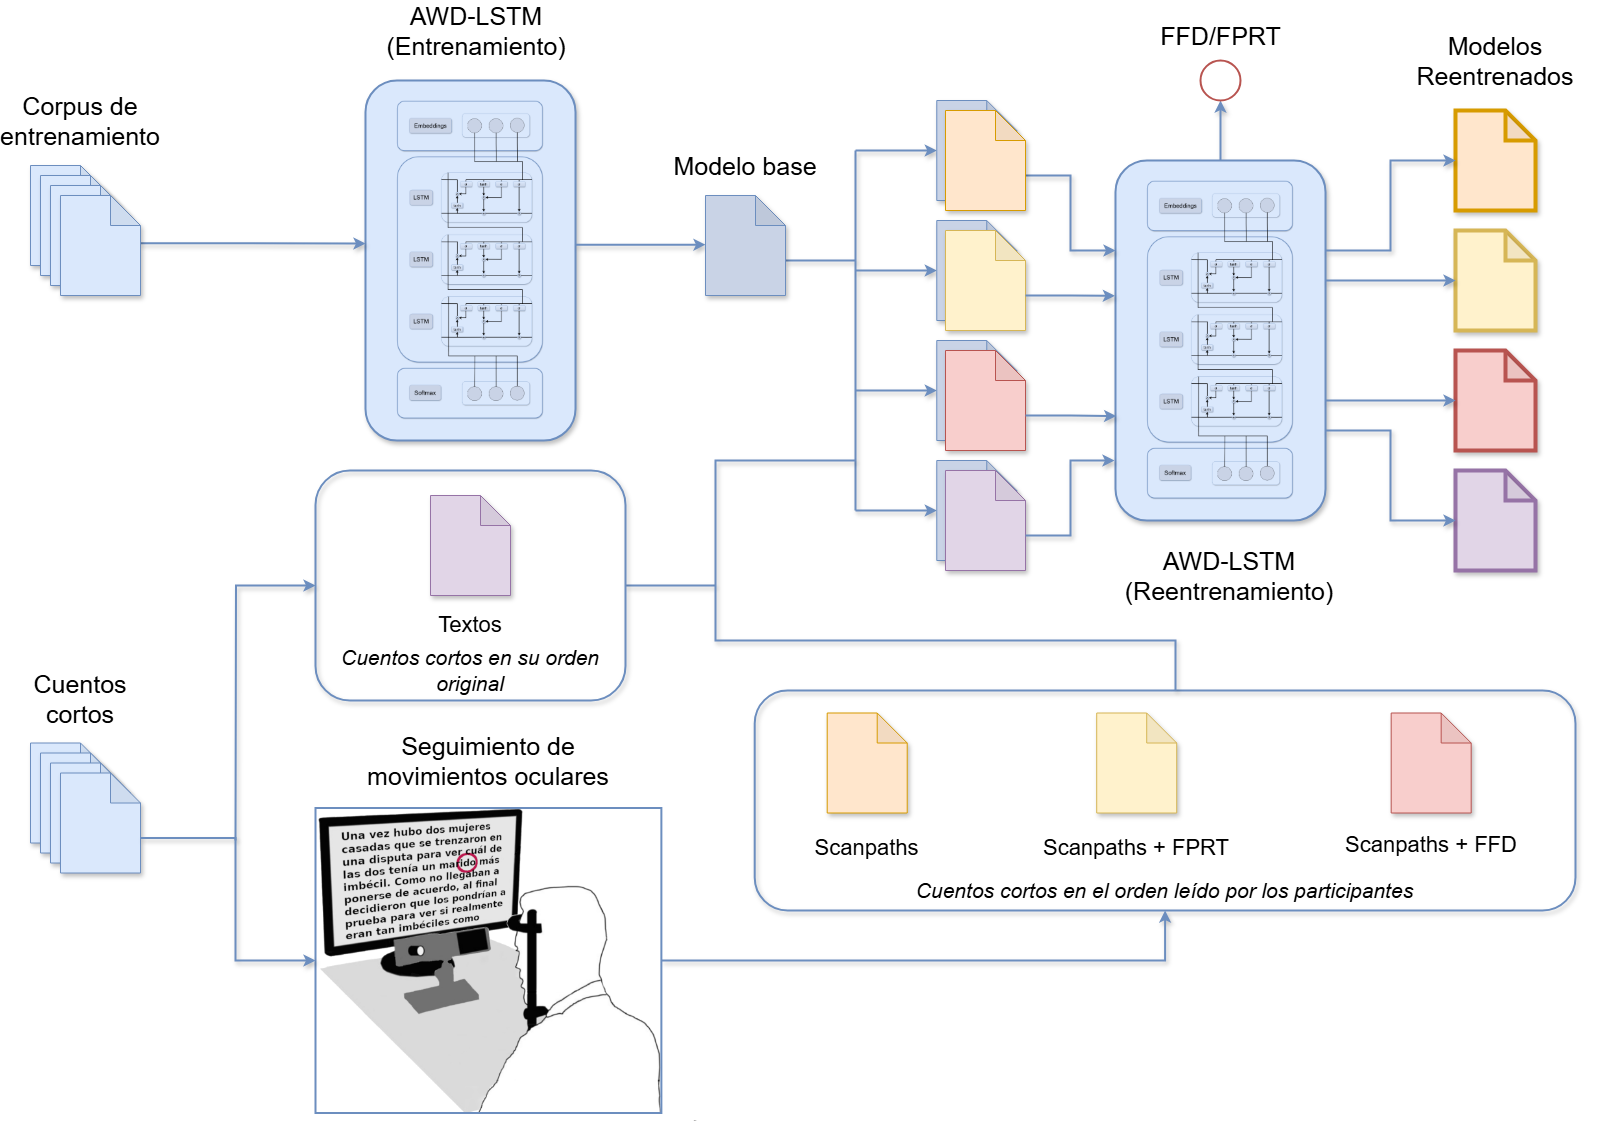
\includegraphics[width=1\textwidth]{imagenes/pipeline.png}
    \caption{Flujo de trabajo durante este proyecto. Se puede observar la generación de los textos basados en los cuentos acompañados con los movimientos oculares para reentrenar un modelo base}
    \label{fig:pipeline}
\end{figure}

\begin{enumerate}
    \item \textit{Textos}: En este caso directamente no se utiliza la información obtenida a partir de los experimentos y solamente se presentan los textos del corpus separados en 1 línea distinta por cada oración.
\end{enumerate}

Para los conjuntos restantes, se decidió utilizar como texto base los \textit{scanpaths} generados por los sujetos durante las pruebas. De esta manera, se puede tener una idea por sujeto de como fue realizándose la lectura de los cuentos. Ahora, para lograr que el modelo AWD-LSTM realice un mejor aprendizaje de las métricas extraídas de estos \textit{scanpaths}, debido a la variedad de valores entre un sujeto y otro, se tomó la decisión de asociar cada palabra dentro de los \textit{scanpaths} con el promedio de las métricas de todos los sujetos en vez de con el valor de la métrica para ese sujeto en particular. Con esto dicho, los conjuntos de reentrenamiento restantes fueron los siguientes:

\begin{enumerate}
    \setcounter{enumi}{1}
    \item \textit{Scanpaths}: Representación de los textos en formato \textit{scanpaths}, sin ninguna métrica en particular que lo acompañe. Por defecto, el valor de la métrica es reemplazado por un 0 para todas las palabras del \textit{scanpath}, pero no se aprende sobre ella.
    \item \textit{Scanpaths\_fprt}: Textos en formato \textit{scanpaths} utilizando la métrica \textit{Gaze Duration} o \textit{First Pass Reading Time}, donde se suman las duraciones de todas las fijaciones en una palabra (antes de salir hacia la derecha o la izquierda).
    \item \textit{Scanpaths\_ffd}: En este caso, los \textit{scanpaths} se ven influenciados por la métrica \textit{First Fixation Duration}, donde solo se conserva la primera fijación en una palabra (antes de salir hacia la derecha o la izquierda).
\end{enumerate}

El objetivo con estos textos es analizar el comportamiento del modelo al añadir información cognitiva, en particular, métricas tempranas sobre los movimientos oculares de los sujetos, las cuales están asociadas entre otras cosas, a la asociación semántica de las palabras.






\chapter{Adaptación de la implementación}

\label{chap:adaptacion}

\section{Implementación Base}

Para poder empezar a adaptar la AWD-LSTM a los requerimientos necesarios, se decidió arrancar con una implementación del modelo de lenguaje obtenida de \textit{GitHub}\footnote{https://github.com/ahmetumutdurmus/awd-lstm}. Esta implementación se eligió frente a otras debido a que esta se encontraba actualizada a las nuevas versiones de la librería \textit{pytorch}, permitiendo así una mejor capacidad de adaptación a las mejoras futuras. En particular el repositorio presentaba una estructura bastante simple, compuesto por 4 archivos principales que daban forma a la arquitectura completa de la AWD-LSTM:

\begin{itemize}
    \item \textit{main.py}: Archivo el cual contenía la lógica del entrenamiento del modelo, permitiendo tunear los hiperparámetros del mismo. Previamente al entrenamiento, en este mismo también se extraían los \textit{datasets} de entrenamiento, testing y validación a partir de importarlos localmente. Luego, estos se dividían en \textit{batches} para poder entrenar al modelo final y validarlo durante las distintas épocas. Para finalizar, el estado del modelo se guardaba cada vez que se lograba encontrar un modelo mejor al finalizar una época. En el caso de que se quisiera interrumpir el script durante el entrenamiento, el código que englobaba al mismo presentaba manejo de excepciones frente a una interrupción voluntaria del usuario, deteniendo el entrenamiento y devolviendo la \textit{perplexity} del último modelo guardado frente al \textit{dataset} de testing.
    \item \textit{finetune.py}: Archivo casi idéntico al anterior, utilizado para reentrenar el modelo en el caso que se preste necesario. Sus principales diferencias recaían en que este archivo permitía inicializar el modelo con alguno ya entrenado previamente, cargando los pesos de la red neuronal a partir de un diccionario que almacenaba el estado de la misma. Además otra característica de este proceso de reentrenamiento es que no estaba implementado de manera que se le pueda indicar al mismo que este reentrene al modelo por una cantidad fija de épocas, sino que él mismo las haría indefinidamente hasta que la condición no monotónica del optimizador se cumpla.
    \item \textit{ntasgd.py}: Archivo el cual definía el optimizador del modelo.
    \item \textit{model.py}: Archivo el cual albergaba todas las clases que en su conjunto representaban a la red neuronal completa que define a la AWD-LSTM. En este mismo se definen todas las capas de la arquitectura, además de especificar cómo se propaga para adelante la entrada de la red, alimentando así los pesos de la misma durante el entrenamiento.
\end{itemize}

Esta implementación presentaba una serie de hiperparámetros los cuales se podían variar para generar distintos modelos de lenguaje. Para más información sobre los mismos o sus valores predeterminados, consultar el anexo. A menos que se indique lo contrario, durante la realización de este trabajo estos serán los valores por defecto que se utilizaran para cada uno de los experimentos.

Por otro lado, yendo más en detalle sobre el archivo \textit{main.py}, en particular sobre de qué manera el programa prepara el corpus de texto para poder alimentar al modelo durante el entrenamiento, se pudo observar que este funciona de una manera un poco particular (Figura \ref{fig:armado_texto}).

\begin{figure}[htb]
    \centering
    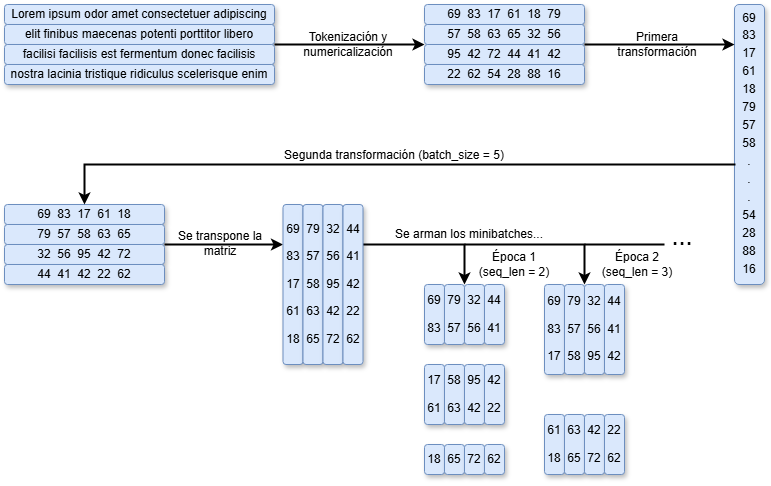
\includegraphics[width=1\textwidth]{imagenes/armado_texto.png}
    \caption{Pipeline usado para generar el \textit{batch} que alimentará al modelo durante el entrenamiento.}
    \label{fig:armado_texto}
\end{figure}

En primer lugar, se separa al corpus de texto en oraciones, donde cada oración se divide en una lista de \textit{tokens}: palabras (sin signos de puntuación, en minúscula, y sin dígitos ni caracteres no romanos) y signos de puntuación, más la introducción de ciertos caracteres extra para brindar más información sobre el contexto de la palabra, desde caracteres que permiten indicar que la palabra siguiente empieza con mayúsculas hasta caracteres que indican el fin de una oración (tokenización). Cada uno de estos \textit{tokens} está representado por un único número (numericalización). Estas listas de números (es decir, las oraciones) son transformadas en un tensor de una única columna con tantas filas como \textit{tokens} haya presentes en la Figura \ref{fig:armado_texto}. Este tensor luego es nuevamente transformado, esta vez en un tensor con una cantidad de filas igual a la cantidad de \textit{batches}. Previamente, con el objetivo de que la cantidad de palabras sea divisible por esta cantidad de lotes y el redimensionamiento del tensor sea posible, se descartaba un pedazo del corpus del final del texto. Una vez hecho esto, se transpone el tensor, quedando una cantidad de columnas igual al tamaño del \textit{batch}.

Por último, para alimentar al modelo, se separan estos \textit{batches} en lotes aún más pequeños, llamados \textit{minibatches}, dependiendo del tamaño de la secuencia que se use en esa época, ya que este tamaño es variable y se recalcula cada vez que se inicia una de ellas \parencite{merity2017regularizingoptimizinglstmlanguage}.

\section{Validación de Implementación Base}

\label{sec:validacion_base}

Una vez presentada la implementación base, se buscó estar seguros de que la misma se comportaba de manera similar en cuanto a capacidad de predicción con una implementación de AWD-LSTM. Para poder averiguar empíricamente esta cuestión, se decidió comparar la implementación base obtenida con la implementación proveída por la librería de \textit{Python} denominada \textit{Fastai}, la cual presenta diversas arquitecturas de modelos de lenguajes. Sin embargo, como esta no permite la modificación de su estructura a nivel red neuronal, se la había descartado como implementación base.
Previamente a esto, se modificó la forma en la cual la LSTM tokeniza y numericaliza los textos, usando también la librería \textit{Fastai} para tokenizarlos, no solo por comodidad, sino también debido a que esta genera nuevos \textit{tokens} de acuerdo a distintos contextos. A futuro esta modificación también serviría en términos de tiempo de ejecución y espacio de memoria, ya que la implementación base obtenía los \textit{tokens} seleccionando el texto completo y transformándolo en un conjunto de palabras, lo cual para corpus muy grandes no sería factible. Los resultados de la comparación se pueden encontrar en la experimentación correspondiente.

Con nuestra implementación empíricamente validada, se continuó la adaptación modificando la forma en la que el modelo recibe el corpus de entrenamiento. En un principio este recibía el corpus a partir de un archivo local. Con el objetivo de poder entrenar la LSTM con textos sustancialmente más grandes en tamaño, lo que se hizo fue adaptar la implementación con una clase llamada \textit{Corpora}, utilizada en trabajos previos en el laboratorio para generar conjuntos de corpus de texto, permitiendo agregar los mismos de manera local o de manera remota a partir de un repositorio de \textit{Huggingface}. De esta manera, sería posible no solo entrenar el modelo con un corpus remoto, como es el caso de \textit{Wikipedia}, sino también reentrenar el modelo con los \textit{scanpaths} generados por los experimentos de movimientos oculares.

Otro cambio que se aplicó a la implementación relacionado a los corpus, fue la eliminación del corpus de testing, para simplificar el código, ya que no lo veíamos pertinente para las experimentaciones futuras. Con esto dicho, en resumidas cuentas para el entrenamiento del modelo la implementación quedó con dos corpus, uno de entrenamiento y otro de validación, correspondientes al 80\% y 20\% del \textit{dataset} original respectivamente. Esta división se hizo de manera aleatoria utilizando una semilla para permitir la replicabilidad de los experimentos en un futuro.

\section{Métricas}
Para poder probar el comportamiento de nuestro modelo a futuro con las experimentaciones, en este trabajo nos hemos centrado en dos métricas generales:

\begin{itemize}
    \item \textit{Perplexity}: La cual se utilizó para medir la capacidad predictiva entre distintos modelos de LSTM, basados en un mismo vocabulario.
    \item \textit{Correlación con juicios de valor humanos}: Utilizando la correlación de \textit{Spearman} y la distancia coseno para averiguar si los \textit{embeddings} generados por la LSTM son capaces de captar las mismas similitudes entre pares de palabras que los capturados por los seres humanos. En caso de querer ver más en detalle cómo se genera esta correlación, ver sección \ref{sec:experimentos_similitud}.
\end{itemize}

Para la primera métrica, la implementación base ya presenta con la capacidad de poder calcular la \textit{perplexity} del modelo a lo largo del entrenamiento. Sin embargo, para obtener la segunda métrica se necesita una manera de obtener \textit{embeddings} a partir de la LSTM. A priori, el modelo no es un modelo dedicado a devolver los \textit{embeddings} de un vocabulario en particular como Word2Vec, sino más bien es un modelo dedicado a predecir la siguiente palabra dado un contexto. Afortunadamente, la arquitectura AWD-LSTM presenta una capa de \textit{embeddings} dentro de la red neuronal, por lo cual el siguiente cambio que se realizó a la arquitectura es el de, una vez finalizado el entrenamiento del modelo, extraer esta capa de \textit{embeddings}, la cual es una matriz de tamaño vocabulario por dimensión del \textit{embedding}, el cual es un hiperparámetro del modelo. 

Una vez extraídos los \textit{embeddings} de la red, estos eran copiados en un archivo de texto en un formato compuesto de la siguiente manera (Figura \ref{fig:archivo_embedding}):

\begin{itemize}
    \item Como primera línea del archivo se encuentran las dimensiones de la capa de \textit{embeddings}.
    \item En las siguientes líneas aparecen, una por cada palabra del vocabulario, la palabra en sí junto a su \textit{embedding}, separadas por un espacio en blanco.
\end{itemize}

\begin{figure}[htb]
    \centering
    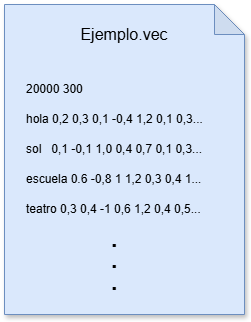
\includegraphics[width=0.35\textwidth]{imagenes/archivo.png}
    \caption{Ejemplo de archivo de texto donde se guardarán los \textit{embeddings} resultante del entrenamiento. En este caso, 20000 sería el tamaño del vocabulario mientras que 300 es el tamaño del \textit{embedding}.}
    \label{fig:archivo_embedding}
\end{figure}

De esta manera, estos \textit{embeddings} pueden ser importados por librerías como \textit{Gensim}, para poder hacer la comparación con otros \textit{embeddings}.

Además, para poder tener una idea más detallada de cómo evolucionan estos \textit{embeddings} a medida que se entrena la LSTM, se tomó la decisión de no solo extraer los \textit{embeddings} finalizado el entrenamiento, sino al terminar cada época del mismo. Luego, estos serían comparados con los juicios de similitud de \textit{Multi-Simlex}, obteniendo la correlación entre los mismos en cada época.

\section{Incorporación de movimientos oculares al modelo}

Como mencionamos previamente, el objetivo principal de este trabajo es el de observar la performance del modelo, luego de añadirle información sobre los movimientos oculares de personas durante la lectura del texto con el cual se está alimentando al mismo. Para poder cumplir esto entonces, se decidió hacer una modificación a la red neuronal clásica de la arquitectura AWD-LSTM. Basados en la idea del aprendizaje multitarea, se tomó la decisión de obligar al modelo a que no solo prediga la siguiente palabra dado un contexto, sino que también prediga las métricas relacionadas con movimientos oculares que más se han estudiado en la literatura: \textit{First Fixation Duration} (FFD) y \textit{First Pass Regression Time} (FPRT, también llamado \textit{Gaze Duration}) (ver \ref{subsec:metricas_movimientos} para su definición).

Yendo más en detalle, se añadió una capa extra en el modelo, compuesta por una regresión lineal, la cual recibe el \textit{batch} con el cual se está alimentando en ese momento a la red y devuelve un resultado. Una vez hecha la predicción, con el objetivo de que la misma vaya mejorando a lo largo de las épocas, se la compara con las métricas reales obtenidas del experimento utilizando el error absoluto medio como función de pérdida. En los casos en donde no existieron métricas relacionadas a movimientos oculares se tomó la decisión de directamente no comparar esta predicción generada, para así no influir en el entrenamiento del resto de la red.

\section{Problemas de memoria}

\subsection{Primera transformación}

Luego de haberse realizado testeos preliminares para asegurar el funcionamiento de la LSTM de manera correcta, el proyecto se topó con un problema importante a solucionar. El código original de la implementación, especialmente en la sección en donde se acondiciona el corpus para transformarlo en un \textit{dataset} adecuado, para luego ser separado en \textit{batches} de texto que serían enviados a la LSTM durante el correr de las épocas, no estaba preparado para poder manejar corpus de gran tamaño. 

Como se mencionó anteriormente, durante la ejecución los corpus eran transformados en un tensor de 1 sola columna y 1 fila por cada palabra que compusiera el mismo, para luego ser nuevamente transformados de acuerdo al tamaño del \textit{batch}. Luego de examinar el código detenidamente, se llegó a la conclusión que existía un problema en esta primera transformación, ya que se hacía utilizando las herramientas básicas del lenguaje de programación y no apoyándose en las librerías externas que dieran un mejor uso de la memoria, haciendo que a medida que se iba generando el tensor, la memoria de la computadora se fuera llenando, llegando a terminar el programa abruptamente cuando el tamaño del corpus era lo suficientemente grande.

Como esto no permitía que la LSTM pudiera ser entrenada con textos extensos, se buscó una manera de mejorar el uso de la memoria en este paso del programa. La solución propuesta fue la de aprovecharse de la interfaz de la librería \textit{Huggingface}, la cual no solo permite la importación de corpus de entrenamiento, sino que también provee una simple interfaz para poder realizar transformaciones sobre el \textit{dataset}, permitiendo así poder replicar la primer transformación del corpus, a la vez de reducir en gran medida el consumo de la memoria en este paso en particular, ya que la herramienta permite ejecutar la transformación de manera paralela dentro de la memoria. Incluso se aprovechó esta herramienta para poder realizar la tokenización y numericalización del corpus, reduciendo no sólo espacio sino tiempo, al también proveer la posibilidad de ejecutar las transformaciones de manera paralela entre varios hilos de ejecución.

Estas modificaciones permitieron que la LSTM se pudiera entrenar con porcentajes cercanos al 30\% de un corpus de texto que contenía alrededor de 28 millones de oraciones. Sin embargo, como los experimentos realizados con otros modelos como Word2Vec se habían llevado a cabo con la totalidad de ese corpus, se decidió probar de entrenar el modelo con un porcentaje mucho mayor.

\subsection{Segunda transformación}

Desafortunadamente, se pudieron observar de vuelta problemas de memoria al entrenar con la totalidad del corpus. Al analizar más en detalle el porqué de esto, nos dimos cuenta que el programa se detenía previo a la segunda transformación mencionada anteriormente, o sea, la que dividía al \textit{dataset} en \textit{batches}. También se encontró un pico de uso de la memoria cuando se accedía al \textit{dataset} en particular, dando la pauta de que el acceso al \textit{dataset} tampoco se estaba haciendo de manera eficiente en este caso.

Un primer enfoque el cual se tomó fue el de recurrir a la librería \textit{PyTorch} y utilizar los \textit{dataloaders} que esta provee, permitiendo un acceso del \textit{dataset} de a \textit{batches} y evitando tener que colocarlo entero en memoria. Esta idea traía un problema crucial: el \textit{dataloader} va generando lotes cuyo texto es contiguo en el corpus, lo cual es evitado en el código original utilizando las transformaciones anteriormente mencionadas, ergo, el conjunto final de \textit{minibatches} resultaba distinto.

Como se buscó mejorar el uso de la memoria del modelo sin alterar íntegramente la lógica del código, se decidió ir por otra solución. Esta solución implicó la utilización de nuevo de la librería \textit{Huggingface} y otro de sus elementos que provee para la alimentación de modelos de lenguaje con corpus de datos extensos, el uso del \textit{sharding} \bb{(Figura \ref{fig:sharding}).}

\begin{figure}[htb]
    \centering
    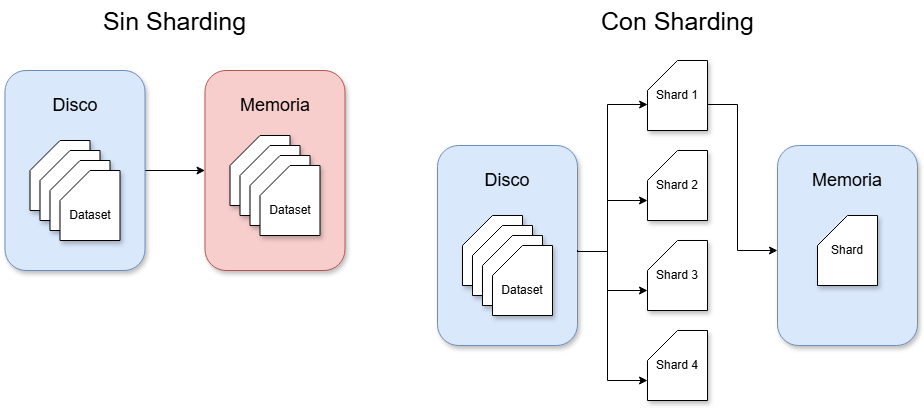
\includegraphics[width=1\textwidth]{imagenes/sharding.png}
    \caption{Sharding, consiste en dividir el \textit{dataset} en fragmentos más pequeños, permitiendo un uso más eficiente de la memoria, ya que lo que ingresa en la memoria es el fragmento y no el \textit{dataset} entero.}
    \label{fig:sharding}
\end{figure}

En particular, en este caso previo a la realización de las transformaciones para generar los \textit{minibatches}, el \textit{dataset} era dividido en una cantidad fija de fragmentos (modificable como parámetro del \textit{script} de entrenamiento), para luego realizar el entrenamiento del modelo de manera normal con el primero de ellos, hasta llegar al último, donde terminado este se daría como finalizada la época. Esto generó mejoras sustanciales en el uso de la memoria, permitiendo el entrenamiento de la LSTM con el 100\% del \textit{dataset} con el uso de 5 fragmentos. No solo eso, sino también permite a futuro poder aumentar la cantidad de fragmentos en el caso de que este modelo se quiera entrenar con un corpus aún más grande.

\subsection{Red neuronal}

Para finalizar, también se hizo una modificación a cómo computa la red neuronal los resultados. En particular, previo a la capa en donde se encuentran las celdas LSTM, se encuentra la capa de \textit{embeddings}, donde el \textit{batch} de palabras que se envían como entrada es transformado en sus respectivos \textit{embeddings}, luego de aplicarse un \textit{dropout} de algunos de estos \textit{embeddings} con el objetivo de reducir el sobreajuste. En esta capa, sin embargo, se descubrió que la manera en que se hacía esto en la implementación original era ciertamente ineficiente en términos de memoria.

\begin{figure}[htb]
    \centering
    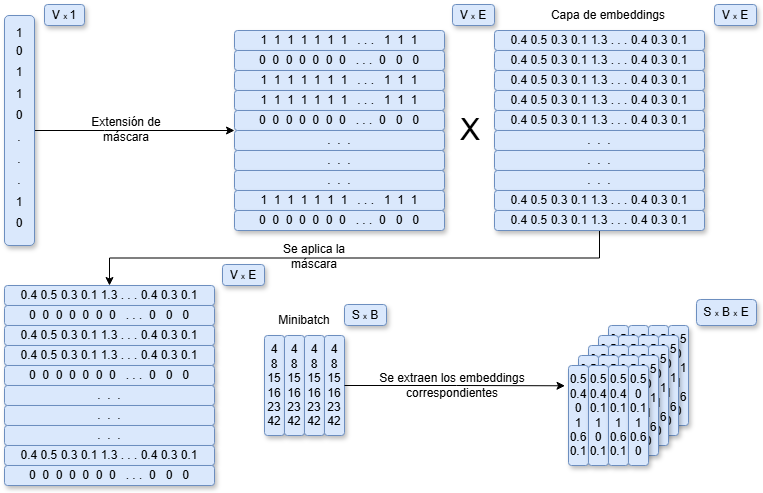
\includegraphics[width=1\textwidth]{imagenes/algoritmo_viejo.png}
    \caption{Algoritmo original para extraer los \textit{embeddings} de la capa de \textit{embeddings}, donde $V$ es el tamaño del vocabulario, $E$ es el tamaño del \textit{embedding}, $B$ es el tamaño del \textit{batch} y $S$ es el largo de la secuencia}
    \label{fig:algoritmo_viejo}
\end{figure}

Para empezar, en la implementación se genera una máscara de una dimensión, del tamaño del vocabulario ($V$), en la cual cada punto corresponde a una palabra en particular y es marcada con un 1 o un 0 de acuerdo a una distribución de bernoulli. Luego esta máscara es extendida a una matriz de dimensión $V + E$ (donde $E$ es el tamaño de los \textit{embeddings}), literalmente copiando los valores anteriores en memoria cuantas veces sean necesarios. No solo eso, además esta máscara es multiplicada celda por celda con la capa de \textit{embeddings} de la red neuronal, deshabilitando algunos \textit{embeddings} de manera aleatoria, pero generando a su vez otra matriz provisoria de tamaño $V + E$. Por último se extraen los \textit{embeddings} de esta matriz provisoria para cada uno de los \textit{tokens} del \textit{batch}. Esta implementación nos pareció ineficiente, especialmente en casos en donde $V$ es grande, pudiendo llegar a ocupar gran parte de la memoria de la GPU innecesariamente (Figura \ref{fig:algoritmo_viejo}).

\begin{figure}[H]
    \centering
    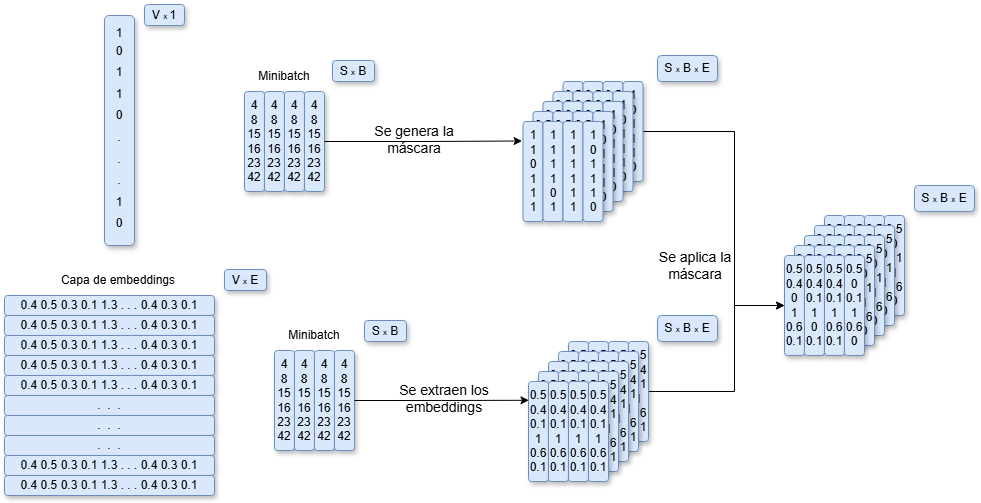
\includegraphics[width=1\textwidth]{imagenes/algoritmo_nuevo.png}
    \caption{Optimización del algoritmo para extraer los \textit{embeddings}. Se definen las mismas variables que en el caso anterior.}
    \label{fig:algoritmo_nuevo}
\end{figure}

Para solucionarlo, se decidió ir por otra implementación más optimizada. En este caso, no se extendió la máscara y se mantuvo como un tensor de una sola dimensión. Luego, directamente se extraen para el \textit{batch} en cuestión los \textit{embeddings} de la capa, generando un tensor de 3 dimensiones, esta vez de tamaño $S \times B \times E$ (donde $S$ es el largo de la secuencia y $B$ el tamaño del \textit{batch}). Además, se genera otro tensor, esta vez solamente de tamaño $S \times B$, donde dentro de él se encuentran los resultados de la máscara para \textit{token} del \textit{batch}, indicando si esa palabra debería ser deshabilitada o no. Por último, se multiplican celda por celda ambos tensores, en definitiva multiplicando ya sea por 1 o por 0 cada uno de los \textit{embeddings} del mismo. Si analizamos detenidamente las dimensiones resultantes de los dos algoritmos, podemos ver, teniendo en cuenta que $S \times B << V$, que los tensores intermedios del segundo algoritmo son mucho más pequeños que los del algoritmo original, ergo ocupando menos espacio de la memoria de la GPU.

\section{Abstracción del código}

Pudiendo ya entrenar sin problemas el modelo con el corpus, se decidió realizar varios cambios estructurales a los archivos con el objetivo de simplificar el código, mejorar la lectura del mismo y poder incorporarlo al sistema original del proyecto, el cual permitía el entrenamiento de otras arquitecturas de manera general, como Word2Vec.

El primero de los cambios fue el de abstraer el código del archivo \textit{main.py} dentro de una clase \textit{AwdLSTM}. Luego, al notar que el código perteneciente al archivo \textit{finetune.py} era idéntico al de su contraparte, se decidió abstraer aún más la clase, transformándola en la interfaz de una jerarquía de clases. Esta jerarquía estaría conformada por una clase \textit{AwdLSTMForFinetuning} y otra llamada \textit{AwdLSTMForTraining}, encargadas del reentrenamiento y entrenamiento del modelo respectivamente. Dentro de estas clases sólo se encuentran las funcionalidades específicas a esa etapa del modelo. Las funcionalidades que se compartan entre estas dos serían englobadas por la interfaz \textit{AwdLSTM}, evitando así código repetido.

Además, aprovechándose de la similitud entre las dos clases, se incorporó polimorfismo a la jerarquía, permitiendo que se simplifique el código aún más al utilizar en funcionalidades que comparten las dos, métodos cuya implementación dependerá del estado del modelo en el que esté. El código se encuentra publicado en \textit{Github}\footnote{https://github.com/FerminT/LMET} para su consulta.

\section{Modificaciones dentro del reentrenamiento}

Una vez ya adaptada toda la etapa de entrenamiento, nuestro siguiente objetivo fue el de modificar la etapa de reentrenamiento para poder arrancar con la experimentación. Un primer cambio fue el de modificar la LSTM para que esta implemente un método estático que funcione como \textit{factory method}, pudiendo así englobar la funcionalidad de generar la clase que define al modelo en un contexto de entrenamiento o en un contexto de finetuning en un solo lugar.
Otra cosa que se hizo fue modificar el criterio de corte del modelo cuando este está finetuneando. En un principio, el reentrenamiento no se hacía durante una cantidad fija de épocas, sino que este terminaba cuando la LSTM alcanzaba la condición no monotónica del optimizador, lo cual con la idea en mente de simplificar el código, se decidió modificar y dejarlo igual a como actúa la LSTM en un contexto de entrenamiento.
Por último, se aseguró que el vocabulario presente en los textos de reentrenamiento estuviera presente en el vocabulario del modelo final. Para eso, en la etapa de entrenamiento se añadió como parte del vocabulario no solo las palabras presentes al corpus de entrenamiento, sino también todas las palabras presentes en el corpus utilizado durante los experimentos de movimientos oculares.




\chapter{Experimentación}

\section{Materiales}

En la presente sección enunciamos los diversos recursos que hemos utilizado y ayudarán a entender cómo se llevaron a cabo los experimentos, tanto previos en el laboratorio como los del presente trabajo.

\subsection{Corpus de entrenamiento}

Para poder entrenar no solo los modelos de lenguaje generados por la AWD-LSTM, 
sino también generar los \textit{embeddings} dentro del modelo de Word2Vec se utilizó un 
corpus grande de texto en español. En particular, se decidió utilizar el corpus 
llamado \textit{all\_wikis}, proveniente del repositorio de textos en español 
\textit{large\_spanish\_corpus}, creado por José Cañete\footnote{https://huggingface.co/datasets/josecannete/large\_spanish\_corpus}.
Este corpus está compuesto por fragmentos extraídos de distintas wikis en español, 
como \textit{Wikipedia}, \textit{Wikinews}, \textit{Wikiquotes} y muchas más, completando un corpus de $28.109.484$ filas, 
correspondiente a una oración por cada una. A menos que se indique lo contrario, 
los modelos serán entrenados con este corpus.

Además, todos los gráficos relacionados a la métrica \textit{perplexity} fueron realizados sobre el \textit{dataset} de validación del corpus, dejando asi el \textit{dataset} de entrenamiento exclusivamente para el entrenamiento de los modelos. Para más informacion sobre como se dividió el corpus, ver la sección \ref{sec:validacion_base}.


\subsection{Experimentos de similitud}

\label{sec:experimentos_similitud}

Como mencionamos anteriormente, el eje principal de este trabajo es el de analizar el 
comportamiento de modelos generados a partir de la arquitectura AWD-LSTM luego de incorporarles 
información cognitiva. Para esto, se decidió comparar los \textit{embeddings} obtenidos de los modelos 
resultantes con dos bases de datos que nos permiten obtener información sobre juicios de similitud 
humanos entre pares de palabras: SWOW-RP y Multi-Simlex. A continuación, se muestra cómo fueron 
preprocesados estos repositorios y de qué manera luego fueron comparados con los \textit{embeddings} 
generados tanto en el presente trabajo como los de trabajos previos en el laboratorio.

\subsubsection{Multi-Simlex}

Como habíamos denotado previamente, Multi-Simlex es un repositorio que cuenta con respuestas 
sobre juicios de similitud entre pares de palabras brindados por 10 anotadores distintos. 
Estos sujetos dieron, para cada par de palabras, un valor de similitud entre $0$ y $6$, donde $0$ 
se considera muy poca similitud y $6$ extremadamente similares. Para poder tener una métrica 
más compacta con la cual comparar los \textit{embeddings}, se decidió tomar el promedio de los valores 
dados por estos anotadores como nuestra medida de similitud final.

Luego, para realizar la comparación con los \textit{embeddings} de los modelos, se calcula la correlación 
de \textit{Spearman} de todos los pares de palabras del repositorio, comparando, por un lado, el promedio 
de los valores dados por estos anotadores y, por el otro, la similitud coseno entre los 
\textit{embeddings} de ambas palabras, extraídos a partir del modelo.

\subsubsection{SWOW-RP}

Por otro lado, SWOW-RP es una base de datos resultante de varias tareas de asociación de palabras provenientes del dialecto rioplatense del español \parencite{Cabana2023}, 
donde a partir de una palabra inicial (\textit{cue}), los sujetos contestaban con las primeras tres 
palabras que se les venían a la mente. A partir de ahí, el repositorio brinda información ya procesada sobre estas tareas, ya sea 
para únicamente la primera respuesta o para las tres. Por ejemplo, brinda la frecuencia de 
una respuesta sobre una \textit{cue} o incluso la probabilidad condicional de haber elegido una 
respuesta a partir de una \textit{cue} en particular. En nuestro caso, se tomó la decisión de tomar 
esta última como medida de similitud entre dos pares de palabras, ya que tomar la frecuencia 
hubiera sido imposible, al tener cantidades distintas de respuestas para cada \textit{cue}. Además se 
eligió contar con la versión de los datos que tiene en cuenta las tres respuestas para mayor 
abarcabilidad.

Luego, para tener una idea más en profundidad del efecto que la información cognitiva puede 
generar sobre los \textit{embeddings}, en este caso se optó por dividir los pares de palabras de este 
repositorio en dos. Por un lado, se agruparon los pares de palabras en donde ambas palabras 
estuvieran presentes en los cuentos; es decir, las palabras que recibieron atributos cognitivos 
durante el reentrenamiento. En el caso de que algunas de las palabras del par no incluyera 
información cognitiva, sería agrupada en el grupo restante.

Por último, se calculó la correlación de \textit{Spearman} de la misma manera que en el caso anterior, 
con la salvedad de que, con el objetivo de obtener mayor rigurosidad estadística, se decidió 
hacer esta comparación no sobre el espacio de pares de palabras total, sino sobre un muestreo 
de $1000$ pares generados con reposición unas $100$ veces.

\section{Trabajos previos}

\label{sec:trabajos_previos}

Previo a este trabajo, dentro del laboratorio de la mano del doctorando Fermin Travi se estuvo 
investigando sobre la incidencia de la información cognitiva sobre otro tipo de modelos previos 
a la arquitectura AWD-LSTM, en este caso, Word2Vec. Haciendo hincapié en el mismo, se utilizó una arquitectura de Word2Vec basada en \textit{skip-grams} y 
se entrenó al modelo utilizando como corpus base el mismo corpus aprovechado en este trabajo, 
valiéndose del 100\% del mismo durante el entrenamiento por una cantidad de 5 épocas.
Luego, los \textit{embeddings} resultantes del modelo fueron comparados con los repositorios de 
juicios de valor humanos presentados anteriormente, calculando la correlación entre los 
\textit{embeddings} y los datos de los repositorios (Figura \ref{fig:simlex_word2vec})

\begin{figure}[htb]
    \centering
    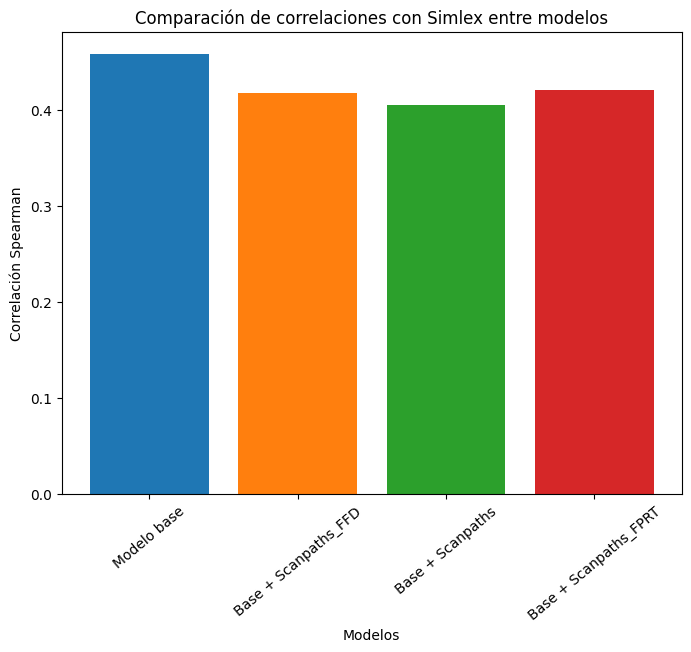
\includegraphics[width=0.6\textwidth]{imagenes/simlex_word2vec.png}
    \caption{Correlaciones entre distintos modelos de Word2Vec con los juicios de valor generados 
    por Multi-Simlex. Entre los modelos comparados se encuentran un modelo base implementado a 
    partir de \textit{skip-grams}, y 3 modelos reentrenados a partir de este, uno con los \textit{scanpaths} sin 
    ninguna métrica asociada y otros dos con los \textit{scanpaths} y las métricas FFD y FPRT asociadas 
    respectivamente.}
    \label{fig:simlex_word2vec}
\end{figure}

En particular, para el caso de Multi-Simlex, el modelo de Word2Vec generado a partir de \textit{skip-grams} 
reportó una correlación de \textit{Spearman} de $0,458$, la cual se utilizará en los experimentos venideros 
como base a la cual comparar los modelos generados por la AWD-LSTM. Además, se evidencia que 
la correlación empeora levemente al reentrenar el modelo con la información cognitiva, lo 
cual se considera esperable que ocurra al haber una gran cantidad de palabras que no se 
vieron influenciadas por el reentrenamiento. Sin embargo, se puede observar que este 
decaimiento es levemente menor en los modelos con las métricas presentes.

\subsection{Reentrenamiento}

Con este modelo base, a su vez, se decidió reentrenar el modelo de \textit{embeddings} 
añadiendo información generada a partir de movimientos oculares, haciendo uso 
de los \textit{scanpaths} generados por los experimentos de información cognitiva. Estos 
fueron reentrenados por una cantidad de 5 épocas valiéndose del 100\% de estos 
textos, introduciendo información sobre los movimientos oculares de los sujetos 
durante la lectura de los mismos.

% Luego, 
Los \textit{embeddings} generados por estos modelos fueron comparados con los datos 
del repositorio SWOW-RP (Figura \ref{fig:swow_word2vec}). Como se puede observar, los modelos reentrenados con los \textit{scanpaths} muestran una peor 
correlación con SWOW-RP comparados con el modelo original, indicando de cierta manera 
que con esta forma de comparación los \textit{embeddings} reentrenados parecen captar peor las 
similitudes entre los pares de palabras obtenidos en el repositorio. Esto al menos, para 
el caso de las palabras en estímulo, o sea las palabras dentro del vocabulario de los 
\textit{scanpaths}. Para el resto de palabras dentro del vocabulario del modelo, no parecen haber 
cambios sustanciales.

\begin{figure}[htb]
    \centering
    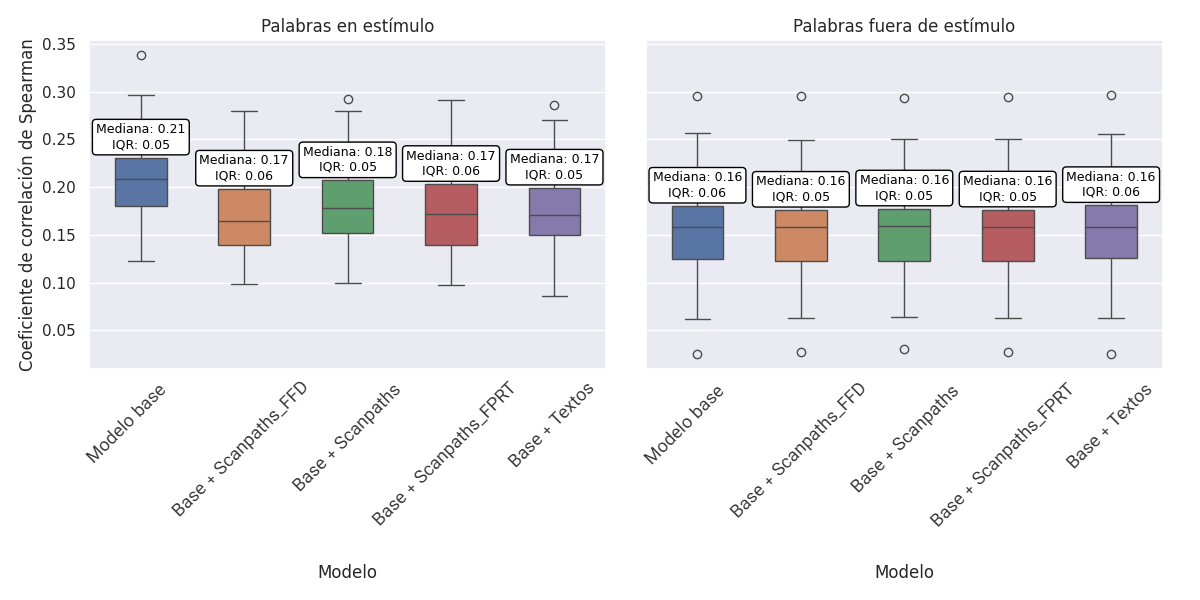
\includegraphics[width=1\textwidth]{imagenes/swow_word2vec.png}
    \caption{Correlaciones entre distintos modelos de Word2Vec y los juicios de similitud 
    generados a partir del repositorio SWOW-RP. La comparación parte con los mismos modelos 
    comparados con Multi-Simlex en la figura \ref{fig:simlex_word2vec}, sin embargo en este caso, se le añade el 
    modelo reentrenado con los textos originales de los cuentos.}
    \label{fig:swow_word2vec}
\end{figure}



\section{Validación de implementación base}

\subsection{Comparación entre implementaciones de AWD-LSTM}

Tal y como se comentó en secciones anteriores, luego de obtener la implementación base 
de la arquitectura AWD-LSTM, se propuso validarla con otra implementación confiable que 
nos permita constatar que el código funciona correctamente. En este caso, se utilizó la 
implementación de la librería \textit{Fastai}.
Para realizar esta comparación, se decidió realizar un experimento entrenando dos 
modelos distintos: uno a partir de la herramienta brindada por \textit{Fastai} y otro 
entrenandolo a partir de la implementación base, con el objetivo de poder corroborar 
que ambos modelos sean parecidos en términos de \textit{performance} (validando empíricamente 
contra la implementación base). Durante el correr de las épocas de entrenamiento de ambos 
modelos, se tomó nota de la \textit{performance}, utilizando la \textit{perplexity} como métrica de los 
mismos frente al dataset de validación. Ambos modelos fueron entrenados utilizando 
uno de los corpus empleados en la experimentación del trabajo original de la AWD-LSTM 
\parencite{merity2017regularizingoptimizinglstmlanguage}, llamado \textit{Penn Treebank Dataset}, el cual engloba una serie de 
artículos en inglés del \textit{Wall Street Journal}, llegando a cubrir una 
cantidad de $38.219$ oraciones.
En particular, ambos modelos fueron entrenados durante $500$ épocas y se los configuró 
de manera tal que los modelos resultantes fueran los más parecidos posibles. Incluso se utilizó el mismo tokenizador, proveniente de la librería \textit{Fastai}, para que el vocabulario 
resultante fuera el mismo y los modelos pudieran ser comparables.

A pesar de esto, debido a las limitaciones de ambas implementaciones, hubo ciertas 
diferencias en la configuración:

\begin{itemize}
    \item Mientras que el \textit{learning rate} del modelo base se mantuvo en su valor por defecto 
    ($30$), en el caso del modelo de Fastai se decidió ejecutar con un \textit{learning rate} 
    de $5\text{e-}3$ (valor recomendado en el ejemplo de uso de la herramienta). Valores mucho más 
    altos, cercanos al \textit{learning rate} de la implementación base, no concluían en resultados 
    satisfactorios, ni siquiera comparables a los del trabajo original.
    \item Por otro lado, mientras que el modelo base se entrenó utilizando como optimizador 
    el algoritmo de NTASGD (ver \textcite{merity2017regularizingoptimizinglstmlanguage}), el modelo de 
    \textit{Fastai} se entrenó utilizando un optimizador ADAM, ya que la librería no presenta 
    dicho optimizador.
\end{itemize}

% \subsubsection{Resultados}

\begin{figure}[htb]
    \centering
    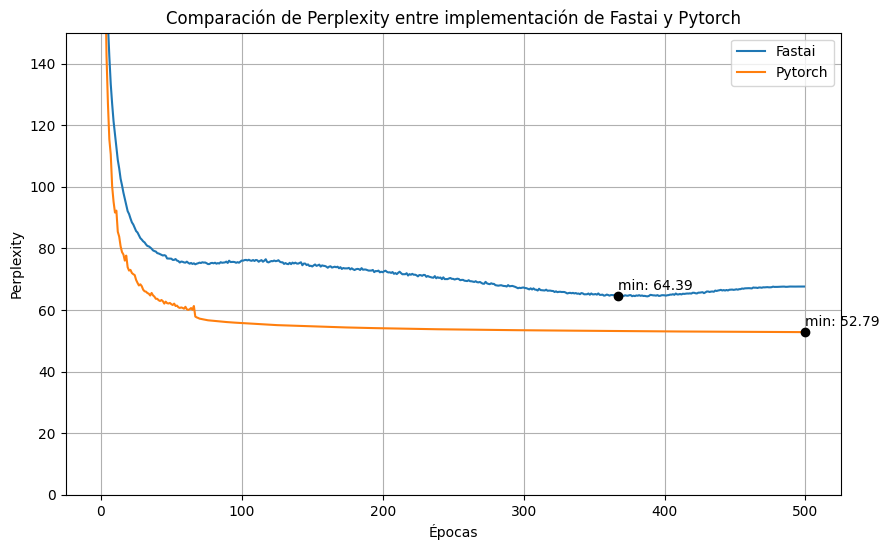
\includegraphics[width=0.8\textwidth]{imagenes/validacion_modelo.png}
    \caption{Comparación de la capacidad predictiva de dos modelos generados a partir 
    de una arquitectura AWD-LSTM a lo largo de las épocas. Uno de ellos fue generado 
    haciendo uso de la librería \textit{Fastai} mientras que el otro fue originado a partir 
    de nuestra implementación base en \textit{Pytorch}.}
    \label{fig:validacion_modelo}
\end{figure}

Como se puede observar en la Figura \ref{fig:validacion_modelo}, con el correr de las épocas, no solo la 
\textit{performance} del modelo base generado en \textit{PyTorch} se asemeja al de su contraparte 
implementado con la librería \textit{Fastai}, sino que también se denota una mejora en la 
\textit{performance} frente a su contraparte a lo largo de las épocas.

% \subsubsection{Síntesis}

A partir de esto, se concluyó que la implementación base de la AWD-LSTM genera resultados 
parecidos al de la implementación generada a partir de herramientas más consolidadas 
como las presentadas por la librería \textit{Fastai}, pudiendo constatar a esta implementación 
como un punto de partida válido para nuestras experimentaciones.

\section{Generación del modelo base}

\label{sec:modelo_base}

Ya contando con nuestra implementación de la AWD-LSTM adaptada a las necesidades de este 
trabajo, para poder cumplir con nuestro objetivo de analizar la performance de la 
arquitectura luego del reentrenamiento con datos provenientes de movimientos oculares 
fue necesario contar con un modelo base.
Para poder obtener el mismo, entrenamos la LSTM con el corpus \textit{all\_wikis} (rejunte de textos 
provenientes de \textit{Wiki-media}) presentado previamente.

\subsection{Comparación con Word2Vec}

Como primer acercamiento para hallar nuestro modelo base, se decidió generar un modelo 
utilizando toda la información brindada por el corpus, sin variar ningún otro hiperparámetro 
en particular. El entrenamiento del mismo se realizó durante 8 épocas y se extrajeron los 
\textit{embeddings} resultantes de la capa correspondiente en la red neuronal.

Luego, se comparó la similitud entre los \textit{embeddings} con la información de los juicios de 
Multi-Simlex al igual que en el caso de Word2Vec, en un principio con la hipótesis de 
poder observar una similitud mayor a los juicios humanos en comparación al modelo previo, 
ya que estamos hablando de una arquitectura posterior en el tiempo.

% \subsubsection{Resultados}

\begin{figure}[htb]
    \centering
    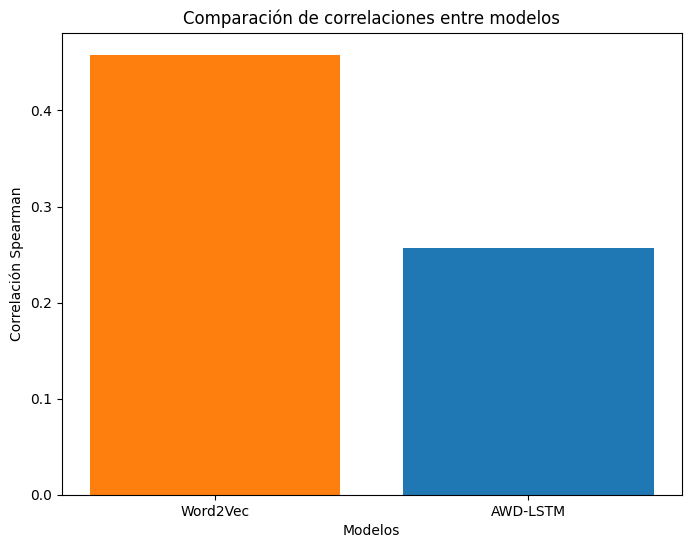
\includegraphics[width=0.5\textwidth]{imagenes/comparacion_w2v_lstm.png}
    \caption{Comparación de correlaciones con Multi-Simlex entre el modelo base 
    generado a partir de Word2Vec y un modelo construido sobre la arquitectura AWD-LSTM, 
    utilizando el 100\% del corpus de entrenamiento.}
    \label{fig:comparacion_w2v_lstm}
\end{figure}

Se puede evidenciar que, al contrario de lo que se suponía, el modelo generado a partir 
de la AWD-LSTM presenta una correlación peor ($0,257$) con los \textit{embeddings} humanos que su 
contraparte generada con Word2Vec ($0,458$), al menos para el caso de Multi-Simlex (Figura \ref{fig:comparacion_w2v_lstm}).

% \subsubsection{Síntesis}

A partir de lo visto, este resultado evidencia (aún de manera no concluyente) que nuestra 
hipótesis inicial sobre la mejor capacidad de captar similitudes entre pares de palabras 
del modelo AWD-LSTM con respecto a Word2Vec podría ser errónea. Sin embargo, 
intuimos a su vez, que será necesario generar otros modelos de AWD-LSTM para tener 
resultados definitivos.

\subsection{Exploración de hiperparámetros}
\subsubsection{Tamaño del Corpus y Épocas}

En vista de los resultados del primer modelo, se tomó la decisión de variar los hiperparámetros 
ligeramente. El primero de ellos que nos interesó variar fue la cantidad de épocas con las 
cuales se entrena al mismo. Sin embargo, esto no nos pareció viable debido al gran tamaño 
del corpus utilizado, ya que esto implicaba un consumo de tiempo muy grande en el entrenamiento 
del modelo, de alrededor de $12$ horas cada época con un tamaño de batch de $30$. Por lo tanto, 
se optó por también reducir el porcentaje del corpus empleado, permitiendo así aumentar la 
cantidad de épocas.

En consecuencia, para el siguiente modelo se decidió permanecer con los mismos hiperparámetros, 
únicamente aumentando la cantidad de épocas de $8$ a $50$ y disminuyendo el porcentaje del corpus 
utilizado de 100\% a 10\%, con el objetivo de observar si la similitud con Multi-Simlex 
aumenta o se mantiene en un número comparable con el modelo anterior.

Adicionalmente, para este experimento calculamos la correlación con los \textit{embeddings} humanos 
al correr de las épocas, junto con la \textit{perplexity}, para ver de qué manera estas evolucionan 
a lo largo del tiempo.

% \subsubsection{Resultados}

\begin{figure}[htb]
    \centering
    \begin{subfigure}[b]{.45\textwidth}
        \centering
        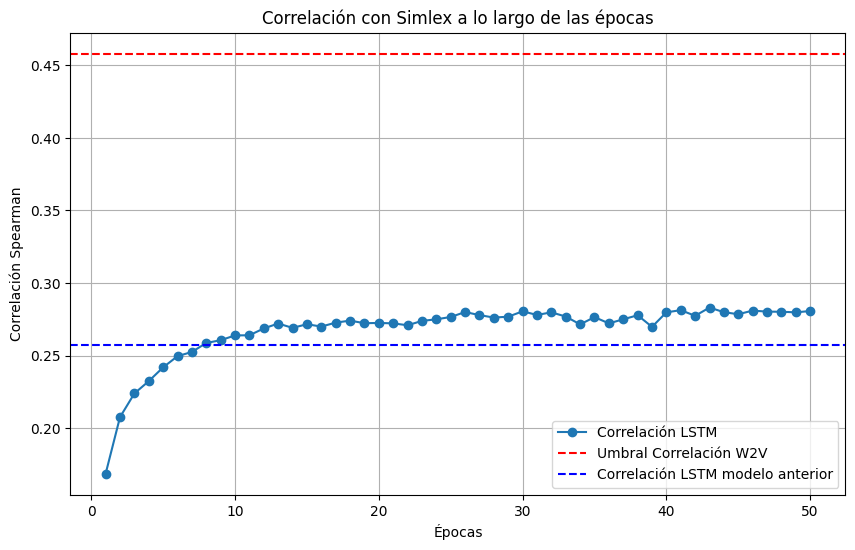
\includegraphics[width=\textwidth]{imagenes/simlex_corr_10per.png}
        \caption{}
        \label{fig:simlex_corr_10per.png}
    \end{subfigure}
    \hfill
    \begin{subfigure}[b]{.45\textwidth}
        \centering
        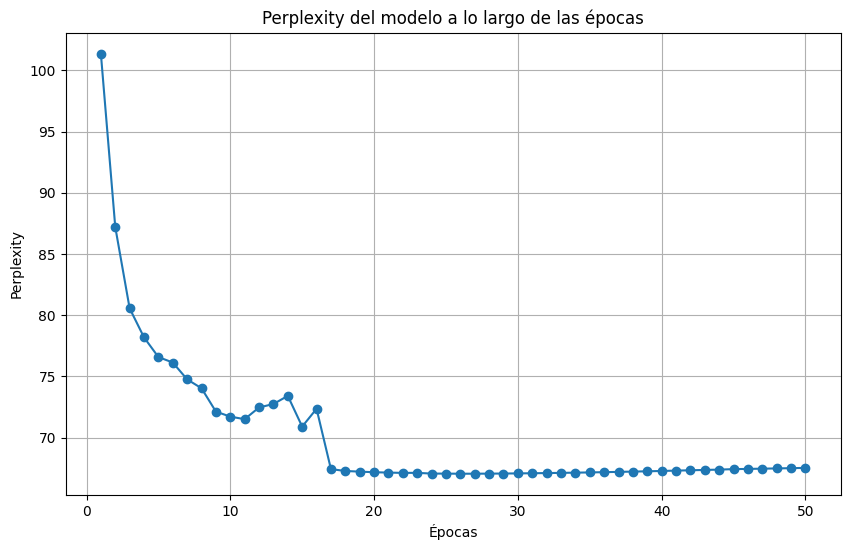
\includegraphics[width=\textwidth]{imagenes/perp_10per.png}
        \caption{}
        \label{fig:perp_10per.png}
    \end{subfigure}
    \caption{En A, correlación con Multi-Simlex a lo largo de las épocas para el modelo con 
    una menor porcentaje de corpus de entrenamiento pero una mayor cantidad de épocas 
    entrenadas. Se grafica consigo la correlación de los modelos de la Figura \ref{fig:comparacion_w2v_lstm} para 
    facilitar la comparación. En B, se grafica la \textit{perplexity} del mismo modelo con el correr 
    de las épocas.}
    \label{fig:10per}
\end{figure}

Dentro del gráfico que mide correlación con Multi-Simlex (Figura \ref{fig:simlex_corr_10per.png}) podemos observar que, 
a pesar de que no se llega a pasar el umbral generado por los resultados con Word2Vec, la 
correlación a lo largo de las épocas termina superando ligeramente aquella del primer 
modelo AWD-LSTM presentado, finalizando el entrenamiento con una correlación de $0,281$.

Por otro lado, la \textit{perplexity} a lo largo de las épocas (Figura \ref{fig:perp_10per.png}) 
evidencia una reducción constante de la misma, mostrando que el modelo está mejorando su 
capacidad predictiva a lo largo de las épocas (al menos hasta la época $17$, donde el 
modelo parece estancarse).

% \subsubsection{Síntesis}

En síntesis, observamos que reducir el tamaño del corpus y aumentar la cantidad de épocas mejoró ligeramente la 
correlación entre los \textit{embeddings}, sin llegar aún al umbral estipulado por Word2Vec. 
Sin embargo, nos permite evidenciar que aumentar el tamaño del corpus no es 
proporcional a la correlación con los juicios de similitud humanos, por lo que 
se tomó la decisión de a partir de ahora seguir insistiendo con un tamaño de 
corpus del 10\% mientras se prueban otras opciones.

% \subsection{Reduciendo el Learning Rate}
\subsubsection{Learning Rate}

Para el siguiente modelo, valiéndose de los resultados anteriores, se eligió reducir el 
\textit{learning rate} que se aplica en el entrenamiento de $30$ a un número menor 
($3\text{e-3}$), con el objetivo de intentar mejorar el aprendizaje del modelo, 
potencialmente evitando el estancamiento de su \textit{perplexity}. En este caso, se decidió 
entrenar el modelo solamente con 25 épocas.

% \subsubsection{Resultados}

\begin{figure}[htb]
    \centering
    \begin{subfigure}[b]{0.45\textwidth}
        \centering
        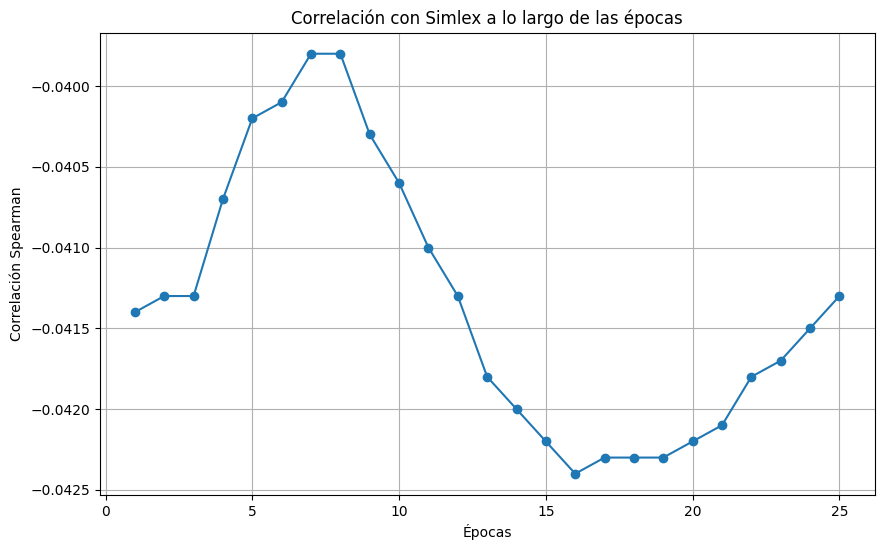
\includegraphics[width=1\textwidth]{imagenes/simlex_corr_lrreducido.png}
        \caption{}
        \label{fig:simlex_corr_lrreducido.png}
    \end{subfigure}
    \hfill
    \begin{subfigure}[b]{0.45\textwidth}
        \centering
        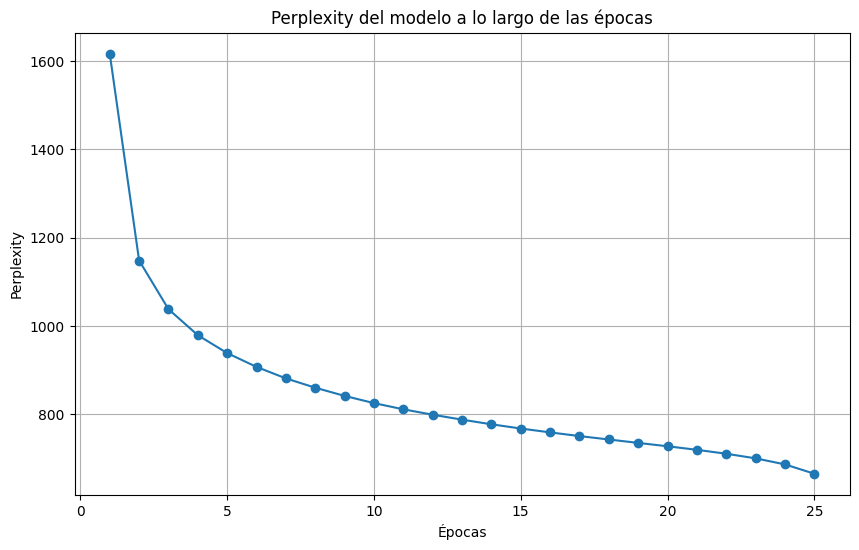
\includegraphics[width=1\textwidth]{imagenes/perp_lrreducido.png}
        \caption{}
        \label{fig:perp_lrreducido.png}
    \end{subfigure}
    \caption{En A, correlación del modelo entrenado con un \textit{learning rate} reducido con 
    Multi-Simlex. Por otro lado, en B se grafica la capacidad predictiva del modelo 
    durante el entrenamiento utilizando la \textit{perplexity} como métrica.}
    \label{fig:lrreducido}
\end{figure}

En lo que a \textit{perplexity} del modelo se refiere (Figura \ref{fig:perp_lrreducido.png}), se puede evidenciar que con un 
\textit{learning rate} menor el modelo no llega a estancarse. Sin embargo, con la cantidad de 
épocas dada no se llega a los niveles de \textit{perplexity} obtenidos en el modelo anterior, 
ya que se observa una mejora lenta de la misma.

Por otro lado, los resultados de la correlación con Multi-Simlex (Figura \ref{fig:simlex_corr_lrreducido.png}) no parecen 
mostrar resultados comparables a los anteriores modelos, posiblemente debido al poco 
aprendizaje realizado por el modelo durante el entrenamiento.

% \subsubsection{Síntesis}

Luego de contemplar los últimos modelos, se puede notar que un \textit{learning rate} como el que 
se utiliza en la LSTM originalmente genera cierto estancamiento en la \textit{performance} del 
modelo, incluso utilizando el algoritmo inherente de la AWD-LSTM que varía el 
\textit{learning rate} de manera aleatoria con el pasar de las épocas. Por otro lado, si 
se reduce este hiperparámetro a un número más estándar dentro de la academia, el 
modelo no se llega a estancar, pero su \textit{performance} no es comparable a la de sus 
predecesores. Con esto en mente, se pensó en modificar la forma en la que varía 
el \textit{learning rate} con el fin de obtener lo mejor de los dos mundos.

% \subsection{Modificación de la variación del Learning Rate}
\subsubsection{Variación del Learning Rate}

A partir de lo mencionado anteriormente, se propuso variar la manera en la que se elige 
el \textit{learning rate} a lo largo de las épocas dentro de la AWD-LSTM. En particular, se tomó 
la decisión de partir del \textit{learning rate} original planteado por la arquitectura e ir 
descendiendo el mismo de manera lineal hasta llegar al utilizado en el experimento 
anterior, buscando que el modelo no se estanque en su capacidad predictiva y sea 
capaz de generar mejores resultados que en los casos anteriores. Adicionalmente, 
se aumentó la cantidad de épocas a $75$ para poder tener más evidencia del estancamiento 
de la \textit{perplexity} del modelo pasadas las épocas. Se compararon los resultados de este modelo con aquellos del modelo que utiliza 
el \textit{learning rate} original ($30$) para poder observar ambas cuestiones.

% \subsubsection{Resultados}

\begin{figure}[htb]
    \centering
    \begin{subfigure}[b]{0.45\textwidth}
        \centering
        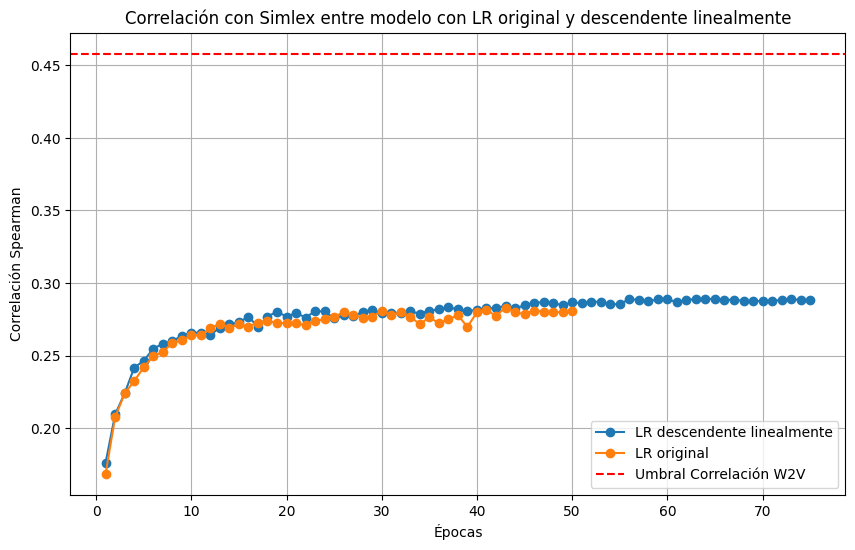
\includegraphics[width=1\textwidth]{imagenes/simlex_corr_lrdescendente.png}
        \caption{}
        \label{fig:simlex_corr_lrdescendente.png}
    \end{subfigure}
    \hfill
    \begin{subfigure}[b]{0.45\textwidth}
        \centering
        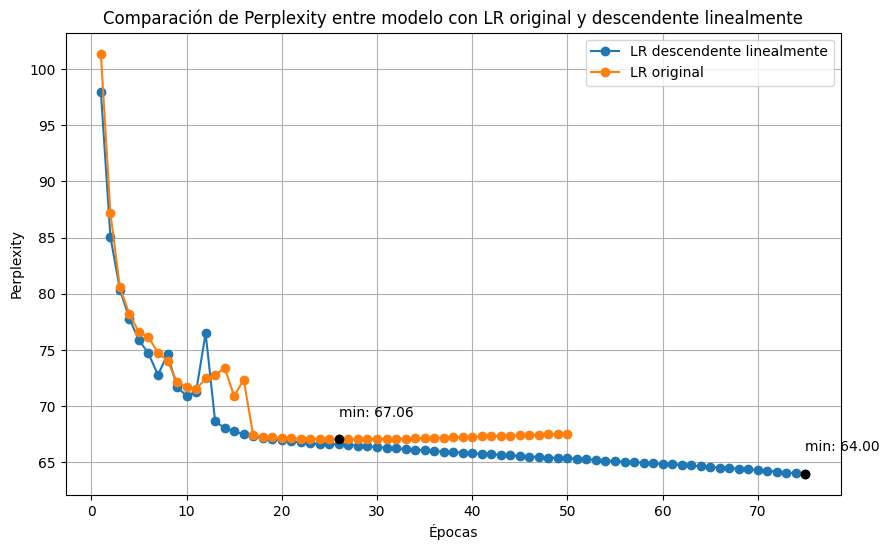
\includegraphics[width=1\textwidth]{imagenes/perp_lr_descendente.png}
        \caption{}
        \label{fig:perp_lr_descendente.png}
    \end{subfigure}
    \caption{Comparación de la correlación con Multi-Simlex a lo largo del entrenamiento 
    entre el modelo de AWD-LSTM presentado en la Figura \ref{fig:10per} y un modelo el cual 
    presenta un \textit{learning rate} el cual desciende linealmente a lo largo de las 
    épocas. En B, se compara la \textit{perplexity} entre ambos modelos.}
    \label{fig:lrdescendente}
\end{figure}

Como se puede observar en la Figura \ref{fig:perp_lr_descendente.png}, mientras que el modelo con el \textit{learning rate} 
original se estanca a partir de una cierta época, el nuevo modelo con el \textit{learning rate} descendiente 
linealmente no solo supera al modelo anterior en \textit{perplexity} dentro de la marca de las $50$ 
épocas, sino que también (al continuar el entrenamiento del modelo) sigue descendiendo 
lentamente gracias a la implementación de un \textit{learning rate} más bajo.

Por otro lado, la correlación con Multi-Simlex del modelo nuevo parece ser idéntica a 
la del modelo anterior, sin presentar mejoras sustanciales. Se puede observar una cierta 
mejora en la correlación en las últimas épocas, pero esto se debe a que el modelo 
nuevo fue entrenado por una cantidad de épocas mayor que el anterior. Incluso 
al compararlo con el umbral obtenido por el modelo de Word2Vec, los resultados 
de los modelos quedan por debajo.

% \subsubsection{Síntesis}

Luego de variar varios hiperparámetros e incluso cambiar la forma en la que se elige 
el \textit{learning rate} del modelo a lo largo de las épocas, no se logró igualar los 
niveles de correlación generados por los \textit{embeddings} de Word2Vec. En vista de esto, 
hipotetizamos que probablemente la diferencia entre ambos modelos no sea un 
tema de los hiperparámetros y su entrenamiento en sí, sino más bien que los 
\textit{embeddings} resultantes de la AWD-LSTM son ciertamente distintos a los 
resultantes del modelo Word2Vec, generando resultados disímiles. También 
es una posibilidad que los valores iniciales de la capa de \textit{embeddings} 
de la AWD-LSTM no ayuden al modelo a converger a los resultados esperados.

\subsection{Embeddings preentrenados}

Para poder poner en evidencia esto último, se optó por realizar un experimento 
adicional previo a la elección del modelo base. Uno de los métodos para ayudar 
a un modelo de lenguaje a mejorar su capacidad predictiva durante el entrenamiento 
es aquella de partir con \textit{embeddings} preentrenados por otro modelo y dejar que 
el modelo actual ajuste estos durante el entrenamiento \parencite{Wang2020}. A partir de esto, se decidió entrenar un modelo idéntico al modelo anterior 
durante $10$ épocas, con la salvedad de que esta vez se lo entrenó inicializando 
la capa de \textit{embeddings} de la red neuronal con los \textit{embeddings} provenientes 
del modelo de Word2Vec.

% \subsubsection{Resultados}

\begin{figure}[htb]
    \centering
    \begin{subfigure}[b]{0.45\textwidth}
        \centering
        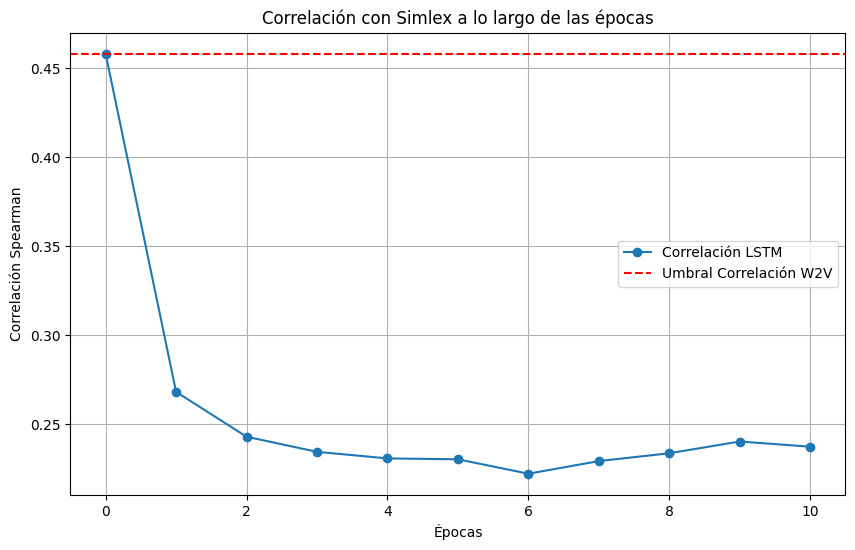
\includegraphics[width=1\textwidth]{imagenes/simlex_corr_preembed.png}
        \caption{}
        \label{fig:simlex_corr_preembed.png}
    \end{subfigure}
    \hfill
    \begin{subfigure}[b]{0.45\textwidth}
        \centering
        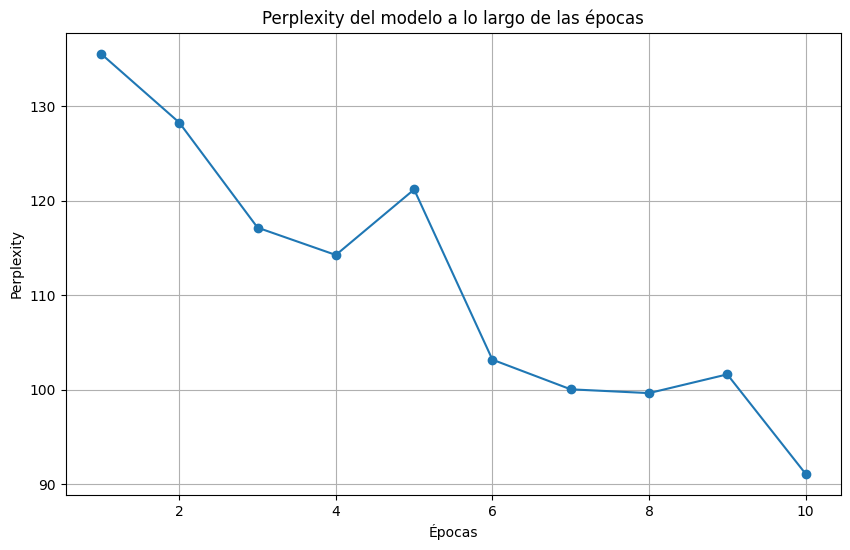
\includegraphics[width=1\textwidth]{imagenes/perp_preembed.png}
        \caption{}
        \label{fig:perp_preembed.png}
    \end{subfigure}
    \caption{En A, se reporta la correlación con Multi-Simlex a lo largo de las épocas 
    del modelo de AWD-LSTM el cual parte de embeddings preentrenados, generados a 
    partir del modelo base de Word2Vec. Nótese que debido a esto, previo al 
    entrenamiento, la correlación con Multi-Simlex es igual que en el modelo 
    de Word2Vec. Por otro lado en B, se reporta la \textit{perplexity} del modelo.}
    \label{fig:preembed}
\end{figure}

Tal y como se puede observar en la Figura \ref{fig:simlex_corr_preembed.png}, la correlación de los 
\textit{embeddings} disminuye drásticamente luego de finalizada la primera época 
de entrenamiento, para luego ir disminuyendo lentamente hasta llegar 
a la época $6$, donde la misma empieza a mejorar levemente. Más aún, también 
se puede observar que la capacidad predictiva del modelo va mejorando 
con el correr de las épocas.

% \subsubsection{Síntesis}

A partir de esta información, se concluye que efectivamente los \textit{embeddings} 
extraídos del modelo resultante de la AWD-LSTM se comportan de una manera 
distinta a los de Word2Vec, evidenciado inicialmente en el brusco decrecimiento 
de la correlación con Multi-Simlex luego de terminada la primer época de 
entrenamiento. El modelo no parece estar aprovechando de ninguna manera 
los \textit{embeddings} preentrenados, transformándolos a lo largo del correr de 
las épocas en \textit{embeddings} parecidos a los generados por la AWD-LSTM.
Por otro lado, al observar que la capacidad predictiva del modelo mejora a 
lo largo de las épocas (al contrario que la similitud con Multi-Simlex) nos da 
la pauta de que estos dos resultados no están correlacionados.

\section{Reentrenamiento del modelo base}

\label{sec:reentrenamiento}
\begin{figure}[htb]
    \centering
    \begin{subfigure}[b]{0.45\textwidth}
        \centering
        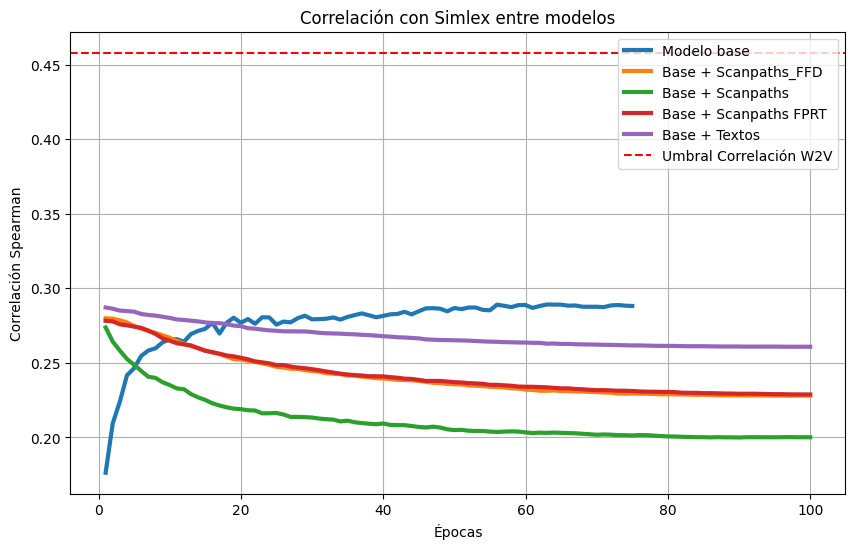
\includegraphics[width=1\textwidth]{imagenes/corr_reentrenamiento.png}
        \caption{}
        \label{fig:corr_reentrenamiento.png}
    \end{subfigure}
    \hfill
    \begin{subfigure}[b]{0.45\textwidth}
        \centering
        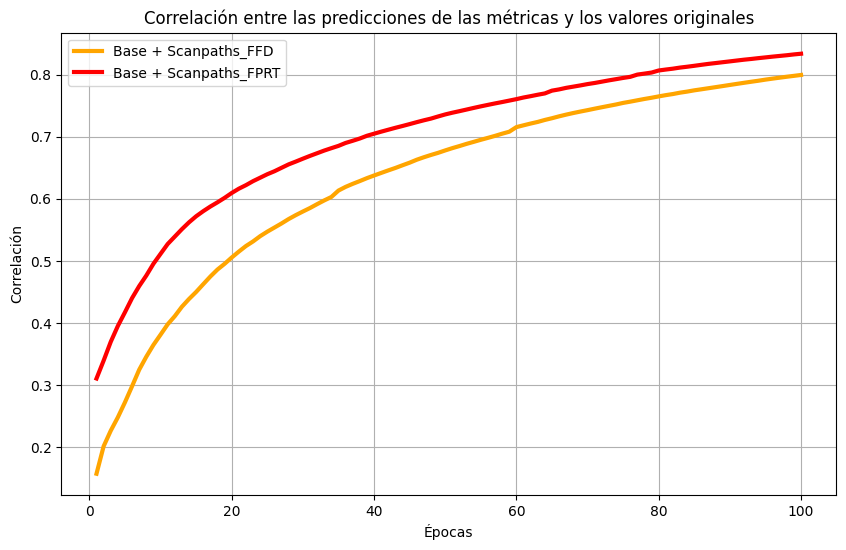
\includegraphics[width=1\textwidth]{imagenes/corr_pred_reentrenamiento.png}
        \caption{}
        \label{fig:corr_pred_reentrenamiento.png}
    \end{subfigure}
    \caption{En A, comparación de la correlación con Multi-Simlex a lo largo de las 
    épocas entre el modelo base elegido y los modelos reentrenados a partir del 
    mismo. En B, para los modelos reentrenados con métricas de movimientos 
    oculares, se reporta la correlación de las predicciones de las métricas 
    generadas por el modelo con los valores originales a lo largo de las épocas.}
    \label{fig:simlex_reentrenamiento}
\end{figure}

Luego de realizadas las experimentaciones pertinentes para lograr hallar un buen 
modelo base sobre el cual reentrenar con información cognitiva, se decidió contar 
con el modelo entrenado a partir de un learning rate linealmente descendente.
A partir de esto, se decidió reentrenar un nuevo modelo utilizándolo como base 
para cada uno de los textos generados a partir de los experimentos con 
movimientos oculares. Estos nuevos modelos fueron reentrenados durante 
$100$ épocas con el 100\% de estos textos, buscando analizar su correspondencia 
con los juicios de similitud humanos utilizados en este trabajo, además 
de compararlos tanto con el modelo base, como con los resultados obtenidos 
en otros modelos, como Word2Vec. En particular, se hicieron comparaciones 
tanto con Multi-Simlex como con SWOW-RP. Para validar el correcto aprendizaje 
de la información cognitiva, también se graficó la correlación de \textit{Spearman} 
entre las predicciones realizadas por el modelo sobre las métricas de 
movimientos oculares para cada época, con el objetivo de ver si los modelos 
lograban aprender a predecir estas métricas a lo largo del entrenamiento.

% \subsection{Resultados}


\begin{figure}[htb]
    \centering
    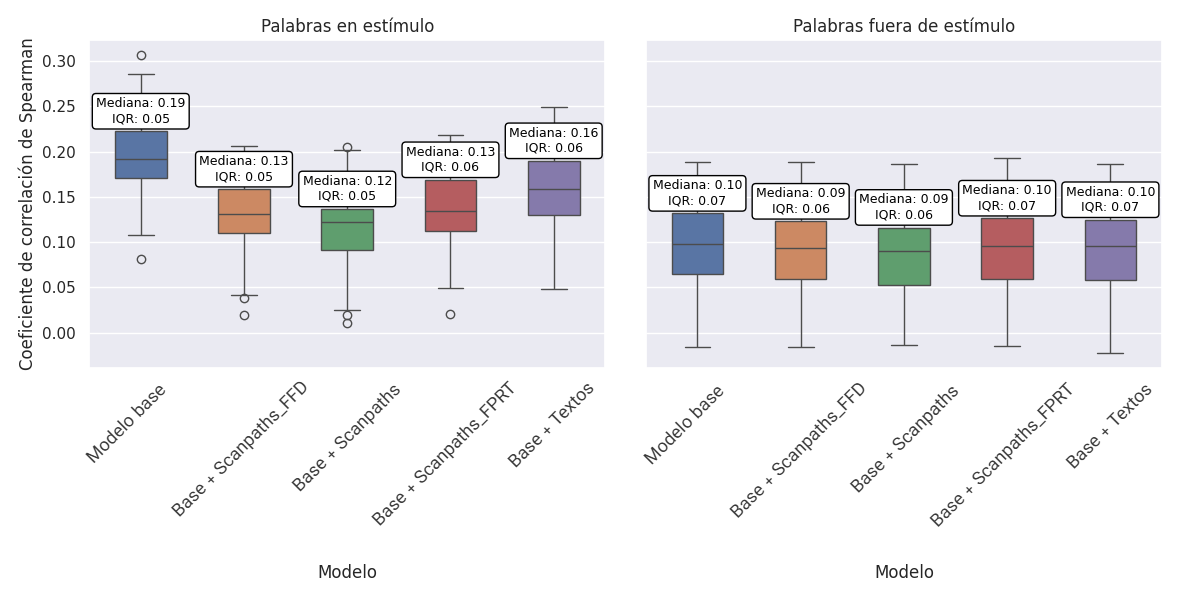
\includegraphics[width=1\textwidth]{imagenes/swow_lstm.png}
    \caption{Comparación de la correlación entre el modelo base y los modelos reentrenados 
    a partir de él con SWOW-RP. Para más rigurosidad estadística, se realiza un 
    muestreo de $1000$ pares de palabras $100$ veces con reposición en vez de 
    comparar todos los pares de palabras una sola vez.}
    \label{fig:swow_lstm}
\end{figure}

A partir de la Figura \ref{fig:corr_reentrenamiento.png} podemos observar que la correlación con Multi-Simlex 
en los modelos reentrenados va disminuyendo paulatinamente a lo largo de 
las épocas, indicando que los \textit{embeddings} generados se van alejando en 
similitud con los datos recabados sobre juicios de similitud humanos. 
Sin embargo, también se puede denotar una diferencia positiva cuando se 
comparan los modelos reentrenados con información cognitiva con el modelo 
reentrenado sin información cognitiva. Por otro lado, en la Figura \ref{fig:corr_pred_reentrenamiento.png}, 
se puede observar que la correlación entre las predicciones de la 
información cognitiva y sus valores originales van aumentando 
considerablemente con el correr de las épocas, dando indicios de que 
el modelo efectivamente está aprendiendo a predecirlas (y, por lo tanto, 
se integran sobre los \textit{embeddings}).

Dentro de la correlación con SWOW-RP podemos hallar resultados parecidos 
(Figura \ref{fig:swow_lstm}), donde la correlación es ciertamente menor en los casos en donde 
el modelo es reentrenado, además de contar con una sutil mejora si a ese 
reentrenamiento se lo acompaña con la información relacionada a los experimentos 
sobre movimientos oculares.
Otro resultado que se puede denotar de esto es que si prestamos atención a 
los resultados sobre SWOW-RP por parte de los modelos de Word2Vec (ver Sección \ref{sec:trabajos_previos}), al igual que en el 
caso que con Multi-Simlex, los \textit{embeddings} provenientes del mismo son más 
capaces de captar las similitudes entre pares de palabras puntuadas por los 
humanos que aquellos provenientes de la AWD-LSTM, aunque en el caso de SWOW-RP 
esta diferencia es menos notoria.

% \subsection{Síntesis}

A partir de lo observado, se puede llegar a la conclusión que dentro de la 
arquitectura AWD-LSTM los embeddings reentrenados con los \textit{scanpaths} 
empeoran la correlación sobre los juicios de similitud humanos utilizados 
en este trabajo. Sin embargo, se puede observar que la reducción de la similitud 
es menor cuando se incorporan a estos textos de reentrenamiento la información 
cognitiva, dándonos la pauta que quizás el problema no se encuentra en la 
información cognitiva sino en el formato del texto de reentrenamiento. 
Esta hipótesis se vuelve más sólida al observar que, durante el reentrenamiento, 
los \textit{embeddings} efectivamente están aprendiendo a predecir las métricas relacionadas 
con los movimientos oculares, incorporando su información.
Más aún, también se puede cuestionar la utilización de la similitud entre 
pares de palabras como la tarea correcta para evaluar a estos modelos, ya 
que su simpleza puede llegar a evitar que se puedan capturar estas 
mejoras obtenidas con la información cognitiva.

\chapter{Conclusiones}

Luego de finalizados los experimentos y puestos en evidencia los resultados de los mismos, 
se decidió partir de dos ejes que se fueron encontrando a lo largo del trabajo para 
elaborar las conclusiones.

El primero de ellos es, al contrario de lo que se esperaba, la diferencia en los 
resultados de las similitudes con los juicios de valor a favor de la arquitectura Word2Vec 
frente a la de la arquitectura AWD-LSTM. Creemos que esto se debe principalmente a la 
estructura interna de estas y a la información que los \textit{embeddings} de cada arquitectura 
albergan dentro de sus dimensiones. Mientras que el objetivo principal de un modelo 
como Word2Vec es devolver una serie de \textit{embeddings}, el objetivo de un modelo de AWD-LSTM 
es aquel de predecir la siguiente palabra dado un contexto. Esto evidencia la necesidad 
de contar con información no sólo semántica de las palabras, sino también sintáctica y 
léxica, información que creemos se encuentra en parte dentro de los \textit{embeddings} de la 
arquitectura, generando así resultados no tan positivos cuando se comparan los mismos 
con juicios de similitud netamente semánticos, como es el caso de Multi-Simlex. 
Por otro lado, se muestra que los \textit{embeddings} generados por Word2Vec 
(\textit{embeddings} cargados de información semántica) obtienen resultados 
considerablemente mejores cuando se comparan con los juicios de similitud humanos.

Esta hipótesis toma más fuerza al observar los resultados del entrenamiento 
con los \textit{embeddings} preentrenados de Word2Vec, ya que desde la primer época 
se ve un descenso brusco de la correlación de los \textit{embeddings} con Multi-Simlex, 
el cual creemos que se debe a que la red neuronal está forzando a los pesos 
de los \textit{embeddings} a cambiar hacia unos \textit{embeddings} con información tanto 
sintáctica como semántica de las palabras dado el contexto de entrenamiento.

Por otro lado, el otro eje, ya haciendo hincapié en la arquitectura AWD-LSTM, es, 
sorpresivamente, la disminución de la similitud con los juicios de valor al 
reentrenar el modelo con textos de los cuentos acompañados con información cognitiva. 
Creemos que esto se debe principalmente a la estructura de los \textit{scanpaths}, los 
cuales al respetar la forma en la que se leyeron los textos, presentando saltos 
de palabras, repeticiones, regresiones, etc, la sintaxis del texto utilizado 
para reentrenar no es sobre lo que fue entrenado previamente el modelo, lo 
que intuimos que empeora los \textit{embeddings} a la hora de compararlos.

Esto se evidencia más al observar que el modelo reentrenado con los textos 
planos es el que mejor similitud presenta frente al resto. De todas formas, 
ninguno de los modelos reentrenados logra superar al modelo base, creemos 
principalmente debido a que la información presente en los cuentos es demasiado 
específica al compararla con el gran corpus de texto con el cual fue entrenado el mismo.

No obstante, también se puede observar que los modelos reentrenados con las 
métricas de movimientos oculares aprenden información sobre las mismas, lo 
cual consideramos que justifica la mejora de la similitud con los juicios de 
valor de los modelos reentrenados con los scanpaths en comparación a su 
reentrenamiento sin dicha información.

Por lo tanto, vemos que existen cabos sueltos que podrían llegar a servir 
de puntapié para trabajos futuros, como por ejemplo:

\begin{itemize}
    \item Cambiar la forma en la cual se incorpora la información cognitiva al modelo, 
    concatenando las métricas \parencite{hollenstein2019} en lugar de 
    predecirlas, condicionando la red neuronal.
    \item Reentrenar el modelo base con otro formato de texto, el cual no 
    conlleve consigo la pérdida de sintaxis de los cuentos y que además 
    permita la incorporación de las métricas.
    \item Evaluar estos embeddings con otros métodos más extrínsecos, 
    como podría ser tareas más relacionadas con el pensamiento humano o 
    subjetividad humana, como análisis de sentimientos o comprensión lectora. 
    Incluso se podrían probar otros métodos de evaluación de la misma 
    índole que los juicios de similitud, como la utilización de 
    analogías de palabras. \parencite{Wang_2019}
\end{itemize}


%%%% BIBLIOGRAFIA
\backmatter
\printbibliography

%%%% El Anexo va al final, dsp de la biblio
\begin{appendices}
    \renewcommand{\thesection}{\Alph{section}} % Use letters for section numbering in appendices
    \addtocontents{toc}{\protect\setcounter{tocdepth}{1}}
    \chapter{Anexo}

    \section{Hiperparámetros del modelo}

    \begin{table}[H]
        \centering
        \begin{tblr}{|>{\centering\arraybackslash}m{4cm}|>{\centering\arraybackslash}m{7cm}|>{\centering\arraybackslash}m{3cm}|}
            \hline
            \textbf{Hiperparámetro} & \textbf{Descripción} & \textbf{Valor por defecto} \\
            \hline
            layer\_num & Cantidad de celdas LSTM que presenta la red neuronal & 3 \\
            \hline
            embed\_size & Tamaño del embedding resultante de la capa de embeddings & 300 \\
            \hline
            hidden\_size & Dimensión del resultado de la capa oculta de la celda LSTM, lo que se conoce como h\_t & 1150 \\
            \hline
            w\_drop & Weight drop correspondiente al interior de la capa de las celdas LSTM & 0.5 \\
            \hline
            dropout\_i & Dropout que se aplica a los vectores de palabras resultantes de la capa de embeddings & 0.4 \\
            \hline
            dropout\_l & Dropout que se aplica entre medio de las conexiones entre una celda LSTM y otra & 0.3 \\
            \hline
            dropout\_o & Dropout que se aplica al resultado de la última capa LSTM & 0.4 \\
            \hline
            dropout\_e & Dropout que se aplica a la capa de embeddings & 0.1 \\
            \hline
            winit & Valor de inicialización de los pesos de la capa de embeddings & 0.1 \\
            \hline
            batch\_size & Tamaño del batch utilizado para entrenar & 30 \\
            \hline
            valid\_batch\_size & Tamaño del batch utilizado para medir performance en el corpus de validación & 10 \\
            \hline
            bptt & Tamaño de la secuencia* utilizado en el algoritmo de backpropagation through time & 70 \\
            \hline
            ar & Parámetro utilizado en el algoritmo de activation regularization & 2 \\
            \hline
            tar & Parámetro utilizado en el algoritmo de temporary activation regularization & 1 \\
            \hline
        \end{tblr}
        \label{tab:hiperparametros_1}
    \end{table}

    \begin{table}[H]
        \centering
        \begin{tblr}{|>{\centering\arraybackslash}m{4cm}|>{\centering\arraybackslash}m{7cm}|>{\centering\arraybackslash}m{3cm}|}
            \hline
            \textbf{Hiperparámetro} & \textbf{Descripción} & \textbf{Valor por defecto} \\
            \hline
            weight\_decay & Constante utilizada en la regularización L2 & 1.2e-6 \\
            \hline
            epochs & Cantidad de épocas & 500 \\
            \hline
            lr & Learning rate & 30 \\
            \hline
            max\_grad\_norm & Threshold utilizado en el algoritmo de gradient clipping & 0.25 \\
            \hline
            non\_mono & Tamaño de la ventana que se utiliza para generar el estado de no monotonicidad & 5 \\
            \hline
        \end{tblr}
        \label{tab:hiperparametros_2}
    \end{table}

    *El tamaño de la secuencia es variable de acuerdo a la época, pero utiliza este valor como base. Para ver mas, consulte en \ref{sec:awd-lstm}


    \begin{scriptsize}
        \begin{sidewaystable}
            \section{Experimentos movimientos oculares}
            \begin{table}[H]
                \centering
                \begin{tblr}{|>
                    {\centering\arraybackslash}m{5cm}|>
                    {\centering\arraybackslash}m{2cm}|>
                    {\centering\arraybackslash}m{2cm}|>
                    {\centering\arraybackslash}m{2cm}|>
                    {\centering\arraybackslash}m{2cm}|>
                    {\centering\arraybackslash}m{2cm}|>
                    {\centering\arraybackslash}m{2cm}|>
                    {\centering\arraybackslash}m{2cm}|>
                    {\centering\arraybackslash}m{2cm}|
                    }
                    \hline
                    Cuento & Autor & Palabras & Fijaciones & Fijaciones Excluidas & Regresiones & Saltos de palabra \\
                    \hline
                    La noche de los feos & Mario Benedetti & 544 & 25774 & 10290 & 8046 & 11234 \\
                    \hline
                    Cómo funcionan los bolsillos & Valentín Muro & 972 & 45815 & 11677 & 16176 & 19705 \\
                    \hline
                    La máscara de la Muerte Roja & Edgar Allan Poe & 572 & 26641 & 6805 & 9092 & 11974 \\
                    \hline
                    Las fotografías & Silvina Ocampo & 618 & 26686 & 8034 & 8580 & 12636 \\
                    \hline
                    La salud de los enfermos & Julio Cortázar & 667 & 34486 & 7596 & 12189 & 17953 \\
                    \hline
                    Buenos Aires & Hernán Casciari & 607 & 28813 & 6855 & 10368 & 12932 \\
                    \hline
                    Wakefield & Nathaniel Hawthorne & 693 & 31610 & 9034 & 10467 & 17397 \\
                    \hline
                    Cómo funciona caminar en la nieve & Valentín Muro & 1066 & 47302 & 10650 & 16245 & 20937 \\
                    \hline
                    Ahora debería reírme, si no estuviera muerto & Angela Carter & 606 & 25629 & 7124 & 7022 & 15558 \\
                    \hline
                    El espejo & Haruki Murakami & 628 & 29851 & 9597 & 9170 & 16788 \\
                    \hline
                    Embarrar la magia & Facundo Alvarez Heduan & 683 & 34749 & 12290 & 12143 & 14400 \\
                    \hline
                \end{tblr}
                \label{tab:experimento_movimientos_oculares_1}
            \end{table}
        \end{sidewaystable}
    \end{scriptsize}

    \begin{scriptsize}
        \begin{sidewaystable}
            \begin{table}[H]
                \centering
                \begin{tblr}{|>
                    {\centering\arraybackslash}m{5cm}|>
                    {\centering\arraybackslash}m{2cm}|>
                    {\centering\arraybackslash}m{2cm}|>
                    {\centering\arraybackslash}m{2cm}|>
                    {\centering\arraybackslash}m{2cm}|>
                    {\centering\arraybackslash}m{2cm}|>
                    {\centering\arraybackslash}m{2cm}|>
                    {\centering\arraybackslash}m{2cm}|>
                    {\centering\arraybackslash}m{2cm}|
                    }
                    \hline
                    Cuento & Autor & Palabras & Fijaciones & Fijaciones Excluidas & Regresiones & Saltos de palabra \\
                    \hline
                    La lluvia de fuego & Leopoldo Lugones & 640 & 30960 & 9236 & 10121 & 15979 \\
                    \hline
                    Educar para escalar y bucear & Andrés Rieznik & 599 & 27797 & 7472 & 9500 & 12621 \\
                    \hline
                    El golpe de gracia & Ambrose Bierce & 602 & 27629 & 7567 & 9540 & 14387 \\
                    \hline
                    La gallina degollada & Horacio Quiroga & 659 & 30188 & 8958 & 9825 & 15769 \\
                    \hline
                    Rubí y el lago danzante & Marcelo Cohen & 641 & 30216 & 8112 & 9332 & 15857 \\
                    \hline
                    La canción que cantábamos todos los días & Luciano Lamberti & 620 & 28299 & 7247 & 8418 & 15386 \\
                    \hline
                    El almohadón de plumas & Horacio Quiroga & 579 & 28063 & 9453 & 8301 & 15087 \\
                    \hline
                    Una rosa para Emilia & William Faulkner & 643 & 33946 & 8968 & 12007 & 16178 \\
                    \hline
                    La de la Obsesión por la Patineta & Hernán Casciari & 579 & 29200 & 8516 & 10044 & 13171 \\
                    \hline
                    \textbf{Total} & - & \textbf{13218} & \textbf{623654} & \textbf{175481} & \textbf{206586} & \textbf{305949} \\
                    \hline
                \end{tblr}
                \label{tab:experimento_movimientos_oculares_2}
            \end{table}
        \end{sidewaystable}
    \end{scriptsize}
\end{appendices}




\end{document}
